%; whizzy chapter
% -initex iniptex -latex platex -format platex -bibtex jbibtex -fmt fmt
% 以上 whizzytex を使用する場合の設定。

%     Tokyo Debian Meeting resources
%     Copyright (C) 2006 Junichi Uekawa

%     This program is free software; you can redistribute it and/or modify
%     it under the terms of the GNU General Public License as published by
%     the Free Software Foundation; either version 2 of the License, or
%     (at your option) any later version.

%     This program is distributed in the hope that it will be useful,
%     but WITHOUT ANY WARRANTY; without even the implied warranty of
%     MERCHANTABILITY or FITNESS FOR A PARTICULAR PURPOSE.  See the
%     GNU General Public License for more details.

%     You should have received a copy of the GNU General Public License
%     along with this program; if not, write to the Free Software
%     Foundation, Inc., 51 Franklin St, Fifth Floor, Boston, MA  02110-1301 USA


%   Pdf作成手順
% dvipdfmx debianmeetingresume200606.dvi
%  preview (shell-command (concat "xpdf " (replace-regexp-in-string "tex$" "pdf"(buffer-file-name)) "&"))
% 画像ファイルを処理するためにはebbを利用してboundingboxを作成。
%(shell-command "cd image200606; ebb *.png")

%%ここからヘッダ開始。

\documentclass[mingoth,a4paper]{jsarticle}
\usepackage[dvipdfmx]{graphicx}
\usepackage{fancybox}
\usepackage{longtable}
\usepackage{ascmac}	% 囲み (screen,itembox)
\usepackage{fancyvrb}   % 囲み Verbatim のために必要
\usepackage[dvipdfmx]{hyperref}
\usepackage{url}
\usepackage[dvipdfmx]{color}
\usepackage{wrapfig} % 図のまわりこみ

%http://www.naney.org/diki/dk/hyperref.html
%日本語EUC系環境の時
\AtBeginDvi{\special{pdf:tounicode EUC-UCS2}}
%シフトJIS系環境の時
%\AtBeginDvi{\special{pdf:tounicode 90ms-RKSJ-UCS2}}

%% spacing の設定をする。外枠を減らす。
\setlength\headheight{0mm}
\setlength\topmargin{-20mm}
\setlength\headsep{0mm}
\setlength\topskip{3mm}
\setlength\maxdepth{4pt}
\setlength\columnsep{6mm}
\setlength\textheight{252mm}
\setlength\topmargin{-5mm}
\setlength\textwidth{170mm}
\setlength\oddsidemargin{-5mm}
\setlength\evensidemargin{-5mm}

% commandline環境を定義。画面入出力についてはcommandline環境
% で表記する
\newenvironment{commandline}%
{\VerbatimEnvironment
  \begin{Sbox}\begin{minipage}{15cm}\begin{fontsize}{7.3}{7.3} \begin{BVerbatim}}%
{\end{BVerbatim}\end{fontsize}\end{minipage}\end{Sbox}
  \setlength{\fboxsep}{8pt}\fbox{\TheSbox}}


%%% start of santaku
\makeatletter
\newwrite\tf@jqz
\immediate\openout\tf@jqz\jobname.jqz\relax
\makeatother
\newcounter{santakucounter}
\newcommand{\santaku}[5]{%
\addtocounter{santakucounter}{1}

\addtocontents{jqz}{\arabic{santakucounter}. #5\\}
\begin{minipage}{1\hsize}
問題\arabic{santakucounter}. 
#1\\
□ A #2\\
□ B #3\\
□ C #4
\end{minipage}
\hspace{1cm}
\\


}
%%% end of santaku

\newcommand{\emptyspace}{(\underline{\hspace{1cm}})}

\newcommand{\subsubsubsection}[1]{%
\vspace{1zw}{\bf #1}\\}

% sectionをセンタリングする
\makeatletter
  \renewcommand{\section}{\@startsection{section}{1}{\z@}%
    {\Cvs \@plus.5\Cdp \@minus.2\Cdp}% 前アキ
    {.5\Cvs \@plus.3\Cdp}% 後アキ
    {\normalfont\Huge\headfont\raggedright\centering}} % style
\makeatother

% section の代わりの環境
\newcommand{\dancersection}[2]{%
\newpage
東京エリアDebian勉強会 2006
\hrule
\vspace{0.5mm}
\hrule
%\hfill{}
\includegraphics[width=3cm]{image200502/openlogo-nd.eps}\\
\hfill{}
\includegraphics[width=16cm]{image2006-natsu/guruguru-sand-light.png}\\
\vspace{-5cm}
\begin{center}
\section{#1}
\end{center}
\hfill{}\colorbox{white}{#2}\hspace{3cm}\space\\
\vspace{1cm}
\hrule
\vspace{0.5mm}
\hrule
\vspace{1cm}
}

% BTSの番号を見るためのコマンド
\newcommand{\debianbug}[1]{#1\footnote{\url{http://bugs.debian.org/#1}}}

% for dancerj
\newcommand{\fgref}[1]{図\ref{#1}}
\newcommand{\tbref}[1]{表\ref{#1}}

\begin{document}

\begin{titlepage}

% 毎月変更する部分
\title{
あんどきゅめんてっどでびあん}
\date{}
\author{\bf 東京エリアDebian勉強会} 
%\maketitle  % use the graphics instead of the text

%%FIXME
\includegraphics[height=252mm]{image2006-fuyu/titlepage-winter.eps}

%\thispagestyle{empty}
\end{titlepage}

\newpage
\setcounter{tocdepth}{1}
\tableofcontents
\vspace{6cm}

\large
\begin{itembox}{\bf『あんどきゅめんてっど でびあん』について}
本書は、東京周辺で毎月行なわれている『東京エリア Debian 勉強会』で
使用された資料・小ネタ・必殺技などを一冊にまとめたものです。
収録範囲は勉強会第18回から第22回まで。
内容は無保証、つっこみなどがあれば勉強会にて。
\end{itembox}
\normalfont

\dancersection{MacBook に Debian をインストール}{上川}
\label{dancerjmacbook}

Apple が2006年春に発売開始した Intel ベースのMacBook に Mac OS X と Debian を
dual-boot でインストールするときの流れを紹介します。

Mac OS X を削除してDebian のみをインストールする方法については、おそらく
liloをMBRから起動するように設定すれば最新ファームウェアは起動してくれま
すが、検証していません。

\subsection{インストール用にパーティション準備}

購入直後の状態では、Mac OS X が全部の領域を占めています。その Mac OS X 
パーティションを縮小し、Debianがインストールできるようにします。Mac OS X
は20GB程度の領域を必要とするようですので、20GBまで縮小してしまいましょう。

diskutil resizevolume コマンドでボリュームサイズを動的に変更することがで
きます。\footnote{resizevolumeコマンドはMac OS X 10.4.6の機能拡張のようです。}

\begin{commandline}
Mac OS X $ df -h
Filesystem                Size   Used  Avail Capacity  Mounted on
/dev/disk0s2               74G    17G    57G    23%    /
devfs                      95K    95K     0B   100%    /dev
fdesc                     1.0K   1.0K     0B   100%    /dev
<volfs>                   512K   512K     0B   100%    /.vol
automount -nsl [171]        0B     0B     0B   100%    /Network
automount -fstab [179]      0B     0B     0B   100%    /automount/Servers
automount -static [179]     0B     0B     0B   100%    /automount/static
/dev/disk0s1              197M   512B   197M     0%    /efi

Mac OS X $ sudo diskutil resizevolume disk0s2 20G
Started resizing on disk disk0s2 Macintosh HD
Verifying

Resizing Volume
Adjusting Partitions

Finished resizing on disk disk0s2 Macintosh HD
WARNING: You must now reboot!

# diskutil list
/dev/disk0
   #:                   type name               size      identifier
   0:  GUID_partition_scheme                    *74.5 GB  disk0
   1:                    EFI                    200.0 MB  disk0s1
   2:              Apple_HFS Macintosh HD       20.0 GB   disk0s2

\end{commandline}

\subsection{rEFItのインストール}

rEFItはEFI専用ブートローダです。
rEFIt\footnote{\url{http://refit.sourceforge.net/} 執筆時点のバージョン
は0.7でした。} イメージを Mac OS X にインストールします。インストールする
場所はどこでもよいのですが、ドキュメントに従ってみましょう。
\texttt{/efi} あたりにファイルを展開し、 rEFIt に含まれている、
\texttt{./enable.sh} を実行します。スクリプト内部で \texttt{bless} コマ
ンド\footnote{EFIでのOS起動優先順序を変更してくれるツール}を実行してくれ
ます。これで、起動時に自動で rEFIt が実行されるようになります。

DebianのrEFItパッケージを利用してインストールする場合には、バージョン0.7-3 
時点では enable.sh が提供されていません。直接blessコマンドを入力してくださ
い。

\texttt{sudo bless --folder \textit{[refit.efiのあるディレクトリへのフルパス]} --file \textit{[refit.efiへのフルパス]}}

\begin{center}
  \includegraphics[width=0.5\hsize]{image200607/bootchain.ps}
\end{center}

\subsection{Debian のインストール}

2006年7月版以降のetch\footnote{これ以前については動作確認をしていません。} 
のインストーラを利用してインストールします。

CDROMから起動するためには、CDROMを挿入してから、Cを押しながら起動すれば
よいです。もしくは、option キーを押しながら起動するとファームウェアの選
択画面が起動します。rEFItのメニューからもCDROMからの起動を選択できます。
\footnote{2006年7月時点でDebian Installer で利用しているLinux カーネル 
2.6.15, 2.6.16 あたりでは Intel Mac に対応できていない問題があり、5回に
4回程度は「APICエラー」なるものが発生し、起動に失敗するので、根気よく起
動するまでがんばってください。2.6.17 以降ではIntel Mac 向けの修正が一部
マージされているので、状況は改善しています。}

パーティションを切る部分\footnote{注意事項としては、既存のEFI FATとMac
OS Xのパーティションは削除しないこと。LILOをインストールする予定のパーティ
ションはパーティション番号 3 か 4 にすること、ということがあります。5番
目以降のパーティションは MBRの制限があるので利用できません。}を過ぎ、パッ
ケージがインストールされたら、LILOをインストールする直前の部分まで実施し
ます。

この時点では LILO が現在動作できない状態になっています。\footnote{parted 
が GPT の仕様に準拠しており、partition 1 のみしかない MBR上のパーティショ
ンテーブルを再作成していることによるようです。}ここで、MBRをGPTに同期さ
せる作業を実施します。ここで、Alt-F2 で仮想コンソールを切替え、コマンド
ラインにうつります。gptsync コマンドを実行してください\footnote{今後はイ
ンストーラから実施できるように改善したいです。}。 現状のインストール方法と
しては、\texttt{chroot /target bin/sh}としてインストール先の chrootに入
り、そこから \texttt{apt-get install refit} でパッケージをインストール、
そして \texttt{gptsync} コマンドでGPTからMBRに同期させます。

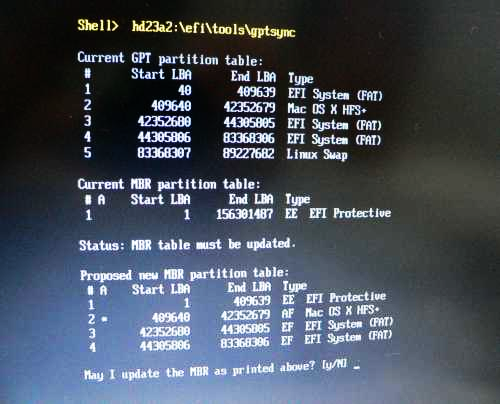
\includegraphics[width=0.9\hsize]{image200607/gptsync.png}

この状態で、インストーラの画面に Alt-F1で戻り、LILO を MBR ではなく、
Linux 用のパーティションにインストールします。再起動するとrEFItからLinux
を指定して起動できるようになっています。

\subsection{各種デバイスの設定}
\subsubsection{Xの設定}

\texttt{X} は \texttt{i810} ドライバで設定します。
\texttt{915resolution} パッケージをインストールします。
解像度は 1280x800 です。

\texttt{/etc/default/915resolution}の例です:\\
\begin{commandline}
#
# 915resolution default
#
# find free modes by  /usr/sbin/915resolution -l
# and set it to MODE
# e.g. use MODE=54 
MODE=32
#
# and set resolutions for the mode.
# e.g. use XRESO=1024 and YRESO=768
XRESO=1280
YRESO=800
#
# We can also set the pixel mode.
# e.g. use BIT=32
# Please note that this is optional,
# you can also leave this value blank.
BIT=
\end{commandline}

xorg.conf の例です\footnote{デフォルトで外部出力もするように設定してあります}:

\begin{commandline}
Section "Files"
	FontPath	"/usr/share/fonts/X11/misc"
	FontPath	"/usr/X11R6/lib/X11/fonts/misc"
	FontPath	"/usr/share/fonts/X11/cyrillic"
	FontPath	"/usr/X11R6/lib/X11/fonts/cyrillic"
	FontPath	"/usr/share/fonts/X11/100dpi/:unscaled"
	FontPath	"/usr/X11R6/lib/X11/fonts/100dpi/:unscaled"
	FontPath	"/usr/share/fonts/X11/75dpi/:unscaled"
	FontPath	"/usr/X11R6/lib/X11/fonts/75dpi/:unscaled"
	FontPath	"/usr/share/fonts/X11/Type1"
	FontPath	"/usr/X11R6/lib/X11/fonts/Type1"
	FontPath	"/usr/share/fonts/X11/100dpi"
	FontPath	"/usr/X11R6/lib/X11/fonts/100dpi"
	FontPath	"/usr/share/fonts/X11/75dpi"
	FontPath	"/usr/X11R6/lib/X11/fonts/75dpi"
	# path to defoma fonts
	FontPath	"/var/lib/defoma/x-ttcidfont-conf.d/dirs/TrueType"
EndSection

Section "Module"
	Load	"i2c"
	Load	"bitmap"
	Load	"ddc"
	Load	"dri"
	Load	"extmod"
	Load	"freetype"
	Load	"glx"
	Load	"int10"
	Load	"type1"
	Load	"vbe"
EndSection


Section "InputDevice"
	Identifier	"Generic Keyboard"
	Driver		"kbd"
	Option		"CoreKeyboard"
	Option		"XkbRules"	"xorg"
	Option		"XkbModel"	"pc104"
	Option		"XkbLayout"	"us"
	Option		"XkbOptions"	"ctrl:nocaps"
EndSection

Section "InputDevice"
	Identifier	"Configured Mouse"
	Driver		"mouse"
	Option		"CorePointer"
	Option		"Device"		"/dev/input/mice"
	Option		"Protocol"		"ExplorerPS/2"
	Option		"Emulate3Buttons"	"true"
EndSection

Section "InputDevice"
	Identifier	"Synaptics Touchpad"
	Driver		"synaptics"
	Option		"SendCoreEvents"	"true"
	Option		"Device"		"/dev/psaux"
	Option		"Protocol"		"auto-dev"
	Option		"HorizScrollDelta"	"0"
EndSection


Section "Device"
	Identifier	"Generic Video Card"
	Driver		"i810"
	Screen		0
	Option "MonitorLayout" "CRT,LFP"
	BusID		"PCI:0:2:0"
EndSection

Section "Device"
	Identifier	"Device1"
	Driver		"i810"
	Screen		1
	Option "MonitorLayout" "CRT,LFP"
	BusID		"PCI:0:2:0"
EndSection

\end{commandline}
\\続く

\begin{commandline}



Section "Monitor"
	Identifier	"Generic Monitor"
	Option		"DPMS"
	HorizSync	28-64
	VertRefresh	43-60
EndSection


Section "Monitor"
	Identifier	"External Monitor"
	Option		"DPMS"
	HorizSync	28-64
	VertRefresh	43-60
EndSection

Section "Screen"
	Identifier	"Default Screen"
	Device		"Generic Video Card"
	Monitor		"Generic Monitor"
	DefaultDepth	24
	SubSection "Display"
		Depth		1
		Modes		"1280x800" "1024x768" "800x600" "640x480"
	EndSubSection
	SubSection "Display"
		Depth		4
		Modes		"1280x800" "1024x768" "800x600" "640x480"
	EndSubSection
	SubSection "Display"
		Depth		8
		Modes		"1280x800" "1024x768" "800x600" "640x480"
	EndSubSection
	SubSection "Display"
		Depth		15
		Modes		"1280x800" "1024x768" "800x600" "640x480"
	EndSubSection
	SubSection "Display"
		Depth		16
		Modes		"1280x800" "1024x768" "800x600" "640x480"
	EndSubSection
	SubSection "Display"
		Depth		24
		Modes		"1280x800" "1024x768" "800x600" "640x480"
	EndSubSection
EndSection

Section "Screen"
	Identifier "Secondary Screen"
	Device "Device1"
	Monitor "External Monitor"
	DefaultDepth 24
	SubSection "Display"
		   Depth 1
		   Modes "1024x768" "800x600"
	EndSubSection
	SubSection "Display"
		   Depth 4
		   Modes "1024x768" "800x600"
	EndSubSection
	SubSection "Display"
		   Depth 8
		   Modes "1024x768" "800x600"
	EndSubSection
	SubSection "Display"
		   Depth 16
		   Modes "1024x768" "800x600"
	EndSubSection
	SubSection "Display"
		   Depth 24
		   Modes "1024x768" "800x600"
	EndSubSection
EndSection

Section "ServerLayout"
	Identifier "Dual-monitor Layout"
	Screen 0 "Default Screen"
	Screen 1 "Secondary Screen" LeftOf "Default Screen"
	# Option "Clone" "On"
	#Option "Xinerama" "On"
	InputDevice "Generic Keyboard"
	InputDevice "Configured Mouse"
	InputDevice "Synaptics Touchpad"
EndSection

Section "DRI"
	Mode	0666
EndSection
 
\end{commandline}

キーバインドは .xsession \footnote{最近はデフォルトでは .gnomerc とい
うファイルが使われるようです。 GDMからデフォルトのシステムセッションを明
示的に選択すれば .xsession を実行してくれるようです。}の中で次のような
設定をしています。右のappleキーを押すと全角・半角キーに割り当てられてい
ます。option と apple キーはよく押し間違えるので、両方を Alt\_Lとして設
定しています。また、イジェクトキーとキーボードの下の部分にあるENTERキー
をマウス用のキーとして定義しています\footnote{xkbsetパッケージが必要。}。
また、外部マウスをUSBで接続した場合も問題なく動作します。

\begin{commandline}
xmodmap -e "keycode 115 = Alt_L"
xmodmap -e "keycode 116 = Zenkaku_Hankaku" # right-apple
xmodmap -e "keycode 108 = Pointer_Button3" # KP-ENTER
xmodmap -e "keycode 204 = Pointer_Button2" # eject
xkbset m
\end{commandline}

\subsubsection{liloの設定}

いつもの癖でboot(/dev/sda3, ext2)とroot(/dev/sda4, ext3)をわけてしまっているのでちょっとややこ
しい例ですが、現在利用しているlilo.conf の例です:

\begin{commandline}
boot=/dev/sda3
root=/dev/sda4
map=/boot/map
delay=20
default=Linux-20060705

image=/boot/vmlinuz-2.6.17dancer-20060701
        label=Linux-20060701
        read-only

image=/boot/vmlinuz-2.6.17dancer
        label=Linux-20060705
        read-only

image=/vmlinuz
        label=Linux
        read-only

image=/vmlinuz.old
        label=LinuxOLD
        read-only
        optional
        initrd=/initrd.img.old

\end{commandline}


デフォルトでインストールされているカーネルが 2.6.17 以前のものであれば、
よく起動時にパニックをおこすので、Intel Mac 対応の 2.6.17 以降のものに
変更しましょう。

\subsubsection{サウンドカード設定}

サウンドカードは \texttt{snd\_hda\_intel} ドライバで対応できる ALSAのオーディオデ
バイスです。

\begin{commandline}
$ cat /proc/asound/cards
 0 [Intel          ]: HDA-Intel - HDA Intel
                      HDA Intel at 0x90440000 irq 50
\end{commandline}

\subsubsection{CPUの動的周波数設定}

cpufreq は \texttt{speedstep\_centrino} で動作します。
apt-get install cpufreqd でインストールして、cpufreqd を動作させてあげ
ると、動作します。

\subsubsection{USBの設定}

USBは UHCI, EHCI です。
通常は特に設定は必要ないはずです。

\subsubsection{電源設定}

バッテリーはまともにサポートしているようです。
ただ、電源の全容量が出ていないので、gnomeから変なメッセージは出ました。

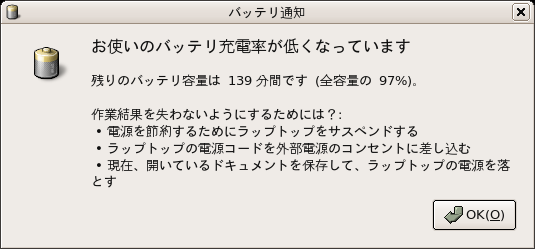
\includegraphics[width=0.8\hsize]{image200607/batterylo.png}

\subsubsection{ネットワークの設定}

有線ネットワークは SKY2 のドライバを利用します。

無線ネットワークは madwifi で対応できます。
インストール方法は下記です。

\begin{itemize}
  \item \texttt{sudo apt-get install madwifi-source madwifi-tools madwifi-doc}
  \item \texttt{sudo m-a prepare}
  \item \texttt{sudo m-a a-i madwifi}
  \item \texttt{sudo modprobe ath\_pci}
\end{itemize}

放っておくとhotplugにより、起動時に自動ロードされて有効になります。
\texttt{/etc/hotplug/blacklist.d/}にファイルを作成し、下記のような内容を
追加しておくと、手動でロードしないと有効にならないようにできます。飛行機に
のる場合などのためには必要かもしれません。

\begin{commandline}
 ath_pci
\end{commandline}

以下、インストール時のログの例です。

\begin{commandline}
 $ sudo apt-get install madwifi-source madwifi-tools madwifi-doc
 $ sudo m-a prepare
Getting source for kernel version: 2.6.17dancer
/lib/modules/2.6.17dancer/source のカーネルヘッダを利用できます
symlink を作成中...
apt-get install build-essential
パッケージリストを読み込んでいます... 完了
依存関係ツリーを作成しています... 完了
以下のパッケージが新たにインストールされます:
  build-essential
アップグレード: 0 個、新規インストール: 1 個、削除: 0 個、保留: 94 個。
6916B のアーカイブを取得する必要があります。
展開後に追加で 20.5kB のディスク容量が消費されます。
取得:1 http://ftp.jp.debian.org sid/main build-essential 11.2 [6916B]
6916B を 0s で取得しました (81.0kB/s)
パッケージフィールドを読み込んでいます... 完了
パッケージ状態を読み込んでいます... 完了
バグレポートを取得しています... 完了
(データベースを読み込んでいます ... 現在 101852 個のファイルとディレクトリがインストールされています。)
(.../build-essential_11.2_i386.deb から) build-essential を展開しています...
build-essential (11.2) を設定しています ...

完了!
$ sudo m-a a-i madwifi
パッケージリストを読み込んでいます... 完了
依存関係ツリーを作成しています... 完了
madwifi-source はすでに最新バージョンです。
アップグレード: 0 個、新規インストール: 0 個、削除: 0 個、保留: 94 個。

1 パッケージについての情報を更新しました
Extracting the package tarball, /usr/src/madwifi.tar.bz2, please wait...
\end{commandline}

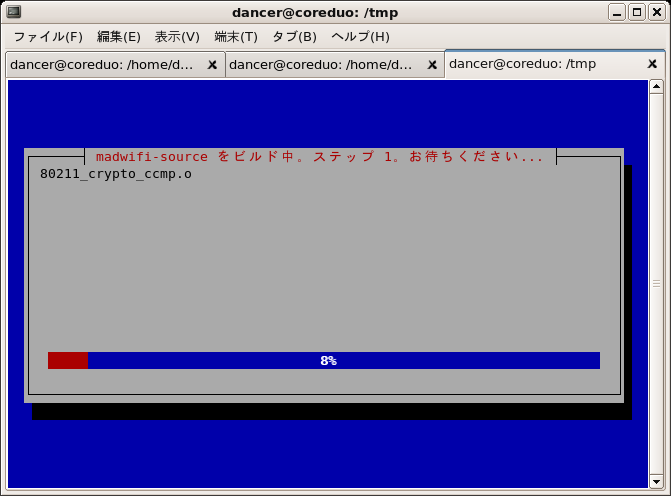
\includegraphics[width=0.8\hsize]{image200607/madwifi.png}

\begin{commandline}
/home/dancer/shared/git/madwifi-modules-2.6.17dancer_0.svnr1644.0.9.0-2+20060705_i386.deb が完了しました。
未選択パッケージ madwifi-modules-2.6.17dancer を選択しています。
(データベースを読み込んでいます ... 現在 101861 個のファイルとディレクトリがインストールされています。)
(.../madwifi-modules-2.6.17dancer_0.svnr1644.0.9.0-2+20060705_i386.deb から) madwifi-modules-2.6.17dancer 
を展開しています...
madwifi-modules-2.6.17dancer (0.svnr1644.0.9.0-2+20060705) を設定しています ...

$ sudo modprobe ath_pci
$ lsmod | grep ath_pci
ath_pci                82212  0
ath_rate_sample        11776  1 ath_pci
wlan                  167132  4 wlan_scan_sta,ath_pci,ath_rate_sample
ath_hal               192208  3 ath_pci,ath_rate_sample
$ dmesg | tail -20
eth1: no IPv6 routers present
ath_hal: module license 'Proprietary' taints kernel.
ath_hal: 0.9.17.2 (AR5210, AR5211, AR5212, RF5111, RF5112, RF2413, RF5413)
wlan: 0.8.4.2 (svn r)
ath_rate_sample: 1.2 (svn r)
ath_pci: 0.9.4.5 (svn r)
Device `[PXS2]is not power manageable<6>ACPI: PCI Interrupt 0000:02:00.0[A] -> GSI 17 (level, low) -> IRQ 169
PCI: Setting latency timer of device 0000:02:00.0 to 64
wifi0: 11a rates: 6Mbps 9Mbps 12Mbps 18Mbps 24Mbps 36Mbps 48Mbps 54Mbps
wifi0: 11b rates: 1Mbps 2Mbps 5.5Mbps 11Mbps
wifi0: 11g rates: 1Mbps 2Mbps 5.5Mbps 11Mbps 6Mbps 9Mbps 12Mbps 18Mbps 24Mbps 36Mbps 48Mbps 54Mbps
wifi0: H/W encryption support: WEP AES AES_CCM TKIP
wifi0: mac 10.3 phy 6.1 radio 10.2
wifi0: Use hw queue 1 for WME_AC_BE traffic
wifi0: Use hw queue 0 for WME_AC_BK traffic
wifi0: Use hw queue 2 for WME_AC_VI traffic
wifi0: Use hw queue 3 for WME_AC_VO traffic
wifi0: Use hw queue 8 for CAB traffic
wifi0: Use hw queue 9 for beacons
wifi0: Atheros 5424: mem=0x90100000, irq=169

$ /sbin/ifconfig ath0
ath0      リンク方法:イーサーネット  ハードウェアアドレス 00:16:CB:BA:76:E7 
          inetアドレス:192.168.22.42 ブロードキャスト:192.168.22.255 マスク:255.255.255.0
          inet6アドレス: fe80::216:cbff:feba:76e7/64 範囲:リンク
          UP BROADCAST RUNNING MULTICAST  MTU:1500  Metric:1
          RX packets:1176 errors:0 dropped:0 overruns:0 frame:0
          TX packets:1607 errors:0 dropped:0 overruns:0 carrier:0
      衝突(Collisions):0 TXキュー長:0 
          RX bytes:230678 (225.2 KiB)  TX bytes:1306390 (1.2 MiB)

\end{commandline}




\subsubsection{リモコン}

赤外線のリモコンは使えるようです。カーネル用のデバイスドライバが存在しま
す。2.6.18以降にとりこまれるのではないでしょうか?
ユーザ空間で利用できるドライバは作成しておきました。
\footnote{\url{http://www.netfort.gr.jp/~dancer/diary/daily/2006-Jul-12.html.ja}}

\subsubsection{iSight}

iSight は linux-uvcデバイスです。
ファームウェアのロードが必要です。
次の手順でインストールができます。

\begin{itemize}
 \item \texttt{apt-get install linux-uvc-tools linux-uvc-source}
 \item \texttt{module-assistant auto-install linux-uvc}
\end{itemize}

アプリケーションはekigaなどを利用しましょう。
v4l2デバイスなので、v4l2対応のソフトウェアが必要です。

\begin{itemize}
 \item \texttt{apt-get install ekiga libpt-plugins-v4l2}
\end{itemize}

実際にロードするには、Mac OS Xのデバイスドライバに入っているファームウェ
アをロードしてからモジュールをロードします。ドライバのある場所のディレク
トリ階層が深いので注意。

\begin{itemize}
 \item \texttt{sudo mount /dev/sda2 /mnt/macosx}
 \item \texttt{sudo macbook-isight-firmware-loader \\
       /mnt/mac/System/Library/Extensions/IOUSBFamily.kext/Contents/PlugIns(次の行に続く)\\/AppleUSBVideoSupport.kext/Contents/MacOS/AppleUSBVideoSupport}
 \item \texttt{modprobe uvcvideo}
\end{itemize}


\subsubsection{未確認のデバイス、手法}

Debianを自動起動させる方法がわかりません、rEFItはデフォルトでは、MacOSX
もしくはeLILOを起動しようとしてしまいます。eLILOを起動すると起動できない。
優先度の変更はどうやったらよいのか、というのがいまいち不明です。

サスペンドの方法。

スリープの方法。

CD-Rの動作はまだ確認していません。PATAパッチが必要という噂です。

\begin{commandline}
 
 # cdrecord -scanbus
 scsibus0:
        0,0,0     0) *
        0,1,0     1) 'ATA     ' 'ST98823AS       ' '7.01' Disk
        0,2,0     2) *
        0,3,0     3) *
        0,4,0     4) *
        0,5,0     5) *
        0,6,0     6) *
        0,7,0     7) *
\end{commandline}

バックライトの制御ができるドライバは作成されているので、2.6.18か19くらい
には入るのではないでしょうか。

bluetoothについては未調査。

\subsection{発表履歴}

本資料は下記の場所での発表資料として作成されたものです。
内容については随時更新しながら、いくつかの場所で発表しています。

\begin{itemize}
 \item 2006年7月2日 秋葉原、CodeFestAkihabara  2006: 最終報告
 \item 2006年7月6日 恵比寿、SGIホール、カーネル読書会: mixi.jp の話の前座
 \item 2006年7月15日 北海道、OSC-Do 2006: 「Debian勉強会」のセッション
 \item 2006年7月29日 日々谷、TLUG: 「MacBookにMac OS XとDebianを
       dual-bootでインストール」
\end{itemize}

\subsection{参考文献}

ファームウェアの bootcamp まわりの開発の影響で、ほとんどのweb上の手順を
書いてある文献は現在の時点で手順が古くなっているので、参考にならない場合
が多いですが、今後更新されるかもしれません。

\begin{itemize}
 \item MacBook Developer Note: MacBookの論理構成図、ハードウェアの概観が解説されています。
       \url{http://developer.apple.com/documentation/HardwareDrivers/Conceptual/MacBook_0605/index.html}
 \item 赤外線リモートコントロール用、IR Receiver パッチ
       \url{http://sourceforge.net/mailarchive/message.php?msg_id=16309282}
       \url{http://www.madingley.org/macmini/kernel/ir.patch}
 \item 赤外線リモートコントロールでXPDFプレゼンテーションするパッチ。
       \url{http://www.netfort.gr.jp/~dancer/diary/daily/2006-Jul-12.html.ja#2006-Jul-12-00:00:06}
 \item MacBook の仕様: 簡単に概要だけが説明されています。
       \url{http://support.apple.com/specs/macbook/macbook.html}
 \item iSight (IEEE1394 外部デバイス)のプログラミングガイド
       \url{http://developer.apple.com/documentation/Hardware/Conceptual/iSightProgGuide/
iSightProgGuide.pdf}
 \item bluetooth のドキュメント: \url{http://developer.apple.com/documentation/HardwareDrivers/Conceptual/HWTech_Bluetooth/index.html#//apple_ref/doc/uid/TP40003032}
 \item mactel linuxのページ \url{http://mactel-linux.org/}、
       ここからたどれるメーリングリストで有用な情報が交換されています。
 \item rEFItのページ \url{http://refit.sourceforge.net/}
 \item \url{http://sharealike.org/index.php?m=200605}
 \item バックライト制御
       \url{http://modular.math.washington.edu/macbook/backlight/}
 \item Ubuntuのインストールについてのまとめページ
       \url{http://desrt.mcmaster.ca/macbook.xhtml}
 \item Gentoo の情報ページ
       \url{http://gentoo-wiki.com/HARDWARE_Apple_MacBook}
 \item MadWifi Wiki
       \url{http://madwifi.org/wiki/UserDocs/Distro/Debian/MadWifing}
 \item Macbook Pro build-in iSight
       \url{http://blogs.gnome.org/view/rbultje/2006/07/08/0}
 \item linux usb video class, linux-uvc
       \url{http://linux-uvc.berlios.de}
 \item Debian wiki MacBook \url{http://wiki.debian.org/MacBook}
\end{itemize}

\dancersection{あなたが知らないうちに使っているDebian specific}{澤田さん}
\label{sec:sawadadebianspecific}

\subsection{はじめに}

Debianパッケージを管理するためのツールであるaptやdpkgなどは一目で
Debian specificとわかります。
しかし、日常的に利用しているコマンド、設定ファイルなど
でも実はDebian固有のものであったり
パッケージ化する際に変更が加えられていたりするものがあります。
ここではそのようなあなたの知らないDebian specificを紹介します。

\subsection{adduser}

Debianで

\begin{commandline}
# adduser hoge
\end{commandline}

を実行するとhogeユーザが作られパスワードの入力が求められます。
Fedoraで同じコマンドラインを実行した場合、hogeユーザは作られますが
パスワード入力は求められません。パスワードは別途passwdコマンドで設定する
必要があります。

この違いはDebianのadduserとFedoraでのadduserの実体の違いによるものです。
Fedoraのadduserはuseraddへのシンボリックリンクです。
DebianのadduserはPerlスクリプトで、useradd、passwd等を
呼び出してユーザを作成しています\footnote{パスワード入力のプロンプトは
passwdコマンドが表示しています}。

ちなみに、FreeBSDのadduserはシェルスクリプトで書かれており、pwというコマ
ンドを呼び出すことでユーザの追加を行っているようです。
Debian GNU/kFreeBSDはFreeBSDカーネルの上にGNUのツールやglibc、Debianのツー
ルを乗せたものであるため、Debianのadduserが使われており、useraddとpasswd
でユーザの追加を行っていました。

\subsection{ifup}

ネットワークの設定を変えたのでインターフェースを再起動したいという場合、
Debianでは以下のコマンドラインを実行するとautoに設定されている
インターフェースをすべて再起動することができます。

\begin{commandline}
# ifdown -a \&\& ifup -a
\end{commandline}

一方Fedoraでは\texttt{-a}オプションは使えず、また、複数のインターフェースを指定す
ることはできません。

インターフェースの設定ファイルもDebianでは\texttt{/etc/network/iterfaces}、
Fedoraでは\texttt{/etc/sysconfig/network-scripts/ifcfg-$<$インターフェース名$>$}
となっており、フォーマットはまったく違います。

\subsection{Xsession}

startxのmanを見るとXの起動時に実行されるスクリプトは\texttt{~/.xinitrc}となって
います。しかし、Debianでは\texttt{~/.xsession}に書いておけばstartxを実行したと
きでもグラフィカルログインしたときでも同じ環境にすることができます。

これは、Debianでは素のXに対して変更を加えているためです。

startxしたときのフローは次のようになっています。
\begin{enumerate}
\item \texttt{/usr/bin/startx}
\item \texttt{~/.xinitrc}があったら\texttt{~/.xinitrc}を実行。なかったら
	  \texttt{/etc/X11/xinit/xinitrc}(Debian向けに修正されています)を実行
\item \texttt{/etc/X11/Xsession}を実行
\end{enumerate}

グラフィカルログイン(xdm)した場合のフローは次のようになります。
\begin{enumerate}
\item \texttt{/etc/X11/xdm/xdm-config}の\texttt{DisplayManager*session}に書かれたコマンド
	  (通常、\texttt{/etc/X11/xdm/Xsession}(Debian向けに修正されています))を実行
\item \texttt{/etc/X11/Xsession}を実行
\end{enumerate}

というわけでどちらの場合も\texttt{/etc/X11/Xsession}が実行されます。
この\texttt{/etc/X11/Xsession}はDebian specificなもので\texttt{/etc/X11/Xsession.d}ディレ
クトリにあるスクリプトを順に実行します。
このうち、\texttt{50x11-common\_determine-startup}で起動プログラムの検出が行われ、
\texttt{~/.xsession}がある場合、\texttt{~/.xsession}が起動プログラムに選ばれます。
\texttt{99x11-common\_start}で\texttt{50x11-common\_determine-startup}で選ばれたプログラム
が実行されることで\texttt{~/.xsession}に書かれた内容が有効になります。

ちなみに、Fedoraでは\texttt{~/.Xclients}に書くとstartxでもグラフィカルログインで
もスクリプトを実行してくれるようです。ただし、\texttt{/etc/X11/Xsession.d}ディレ
クトリのような仕組みはないようです。

\subsection{lesspipe}

lessでgzip圧縮されたファイルを開こうとすると通常次のようになります。

\begin{commandline}
$ less hoge.txt.gz
"hoge.txt.gz" may be a binary file.  See it anyway?
\end{commandline}

ひょっとしたら上のようなメッセージは表示されずに
hoge.txtの内容が表示されている方もいらっしゃるかもしれません。
その場合、次の環境変数が設定されているはずです。

\begin{commandline}
$ printenv | grep ^LESS
LESS=-M
LESSOPEN=| /usr/bin/lesspipe '%s'
LESSCLOSE=/usr/bin/lesspipe '%s' '%s'
\end{commandline}

lessには\texttt{LESSOPEN}という環境変数が設定されているとファイルを読み込む前
に\texttt{LESSOPEN}で指定されたコマンドにファイル名を渡してコマンドの標準出力をファ
イルの内容として読み込むという機能があります。
これにより、gzip圧縮されたファイルを

\begin{commandline}
$ less hoge.txt.gz
\end{commandline}

というコマンドラインで表示することができます。
また、この機能を応用することで

\begin{commandline}
$ less hoge.tar.gz
\end{commandline}

とした場合にtarされているファイルの一覧を取得するといったこともできます。

\texttt{/usr/bin/lesspipe}はDebian specificなものです。他のディストリビューション
にも同様の機能を持つものが含まれていることが多いのですが、Debianの
lesspipeは対応している拡張子の数が多いことが特徴です。

language-envを実行すると\texttt{LESSOPEN}の設定をしてくれるため
気づかず使っているという方もいらっしゃるのではないでしょうか。

\subsection{Debian specificの見つけ方}

それがDebian specificであるか知るためにはmanを参照するという方法がありま
す。manを見ると、

\begin{commandline}
Debian GNU/Linux        Version 3.97        ADDUSER(8)
\end{commandline}

のように書かれているのでDebian specificと推測することができます。
しかし、それ以外にDebian specificかを知るよい方法はないようです。

Xsessionやlesspipeのようにオリジナルの配布内容からファイルが追加されてい
る場合、ソースパッケージのdebianディレクトリに追加ファイルが格納されてい
ます。
debianディレクトリにあるファイルリストからcontrolやpostinstなどの制御ファ
イルを除いたものを取得すればそのパッケージにDebian specificな変更があり
そうか推測することができると考えられます。

%% さわださんここまで
%% 小林さんここから
\dancersection{翻訳へのさそい}{小林さん}
\label{sec:honnyaku}

\subsection{はじめに}

国際化はDebianの一つの特徴です。
その国際化の達成には、
フレームワークの整備から各ソフトウェアの対応、
そしてメッセージやドキュメントの翻訳まで、
多岐に渡る非常に膨大な作業を必要とします。
ここでは、それらの作業のうち、
最も大量の作業を必要とする一方で一般ユーザが最も取り組みやすい翻訳に
ついて、
主にDebian JPまわりで行われている日本語訳作業をまとめます。

\subsection{共通の作業用インフラストラクチャ}

まず、
翻訳作業で共通に使われるインフラストラクチャをまとめて説明します。
これらは、後述する各種作業の説明でも頻繁に登場します。

\subsubsection{作業用メーリングリスト}

翻訳作業に関するやりとりには主にメーリングリストが使われます。
Debian本家のものとDebian JPのものがありますが、どちらについても、
翻訳関連のメーリングリストは誰でも (DebianおよびDebian JPのメンバーで
なくても) 自由に参加できます。

日本語訳関連の作業に関するやりとりによく使われるのは、
Debian JPのdebian-doc\footnote{\texttt{debian-doc@debian.or.jp}}および
debian-www\footnote{\texttt{debian-www@debian.or.jp}}メーリングリストです。
登録に使うアドレスは、
それぞれ\texttt{debian-doc-ctl@debian.or.jp}と
\texttt{debian-www-ctl@debian.or.jp}です。
これらのメーリングリストに関する情報が、
\url{http://www.debian.or.jp/MailingList.html}\footnote{%
準備中の新サイトでは
\url{http://www-internal.debian.or.jp/community/ml/}。}にあるので、
参照してください。
過去にこれらのメーリングリストに投稿されたメールのアーカイブは、
\url{http://lists.debian.or.jp/debian-doc/}および
\url{http://lists.debian.or.jp/debian-www/}で完全に公開されています。

さらに、パッケージの更新に伴うdebconf-poの翻訳更新の依頼など、
Debian本家の開発者との英語でのやりとりには、
主にDebian本家のdebian-japaneseメーリングリスト\footnote{%
\texttt{debian-japanese@lists.debian.org}}が使われます。
登録およびアーカイブは\url{http://lists.debian.org/debian-japanese/}で
利用可能です。
メーリングリストを経由せずに、前のバージョンの翻訳者や、
翻訳者として活発に活動されているかた、
あるいは本家で活動している日本人開発者のところに直接メールが行ったりする
こともあります。

また、
ドキュメントの翻訳ならDebian本家のdebian-docメーリングリスト\footnote{%
\texttt{debian-doc@lists.debian.org}}に、
ウェブページの翻訳ならDebian本家のdebian-wwwメーリングリスト\footnote{%
\texttt{debian-www@lists.debian.org}}にそれぞれ登録しておくと、
内容に関する質問や間違いの修正などに関するやりとりを本家の方々とできます。
それぞれ\url{http://lists.debian.org/debian-doc/}および
\url{http://lists.debian.org/debian-www/}で、
登録やアーカイブ閲覧ができます。

\subsubsection{対訳表}

日本語訳の対訳表は、Debian JP debian-docメーリングリストでたまに
話題になりますが、なかなか整備までいかないのが現状です。
メーリングリストで訳語に関する問い合わせをしたり、
査読依頼を出してコメントをもらったりできるので、
そこまで気になることはないでしょう。
一応、既存のいくつかの対訳表をポインタとして示しておきます。
\begin{itemize}
 \item Debian JPの『略語の解説』:
       \url{http://www.debian.or.jp/devel/abbreviation.html}
 \item Debian JP対訳表
       \begin{itemize}
	\item ソース: \url{http://www.debian.or.jp/Documents/trans_table/}
	\item HTMLでの出力:
	      \url{http://www.debian.or.jp/Documents/trans_table/trans_table.html}
	\item dict形式での出力:
	      \url{http://www.debian.or.jp/Documents/trans_table/trans_table.dict}
       \end{itemize}
 \item APT, dpkg関連の表記に関する用語集 (武藤健志さんのWiki):
       \url{http://kmuto.jp/open.cgi?DebianGlossary}
 \item かねこさんによる『Security関連用語対訳集』:
       \url{http://lists.debian.or.jp/debian-www/200607/msg00120.html}
 \item 小林によるDebian Weekly News関連のja.po\footnote{Debian Weekly
       News用wmlファイルの後半のSecurity UpdatesおよびRemoved Packagesから
       用語を抽出してpoとしたものです。}:
       \url{http://dolphin.c.u-tokyo.ac.jp/~nori1/dwn/ja.po}
\end{itemize}

対訳表というわけではありませんが、
これらの他に小林が訳語の選択によく利用するのは、Googleです。
Debianのウェブサイト全般から訳語を探したければ「site:www.debian.org」を、
Debian Weekly Newsから探したければ「site:www.debian.org/News/weekly」を
つけて検索し、引っ掛かったページを見ながら訳語を決めるということをよく
やっています。

\subsection{各種ソフトウェアのpoや付属ドキュメントの翻訳}

\subsubsection{作業方法}

各種ソフトウェアのメッセージカタログ (po) や付属ドキュメント、
manpageなどの翻訳に関する議論は、
Debian JPのdebian-docメーリングリストで行われています。
これらの翻訳はソフトウェアの更新に伴って更新作業をする必要があるので、
主に開発元 (upstream) のソフトウェア作者などと (主に英語で) やりとりを
しながら作業することになります。
しかし、特にDebianと密接に関連したソフトウェアについては訳語が統一されて
いるほうがよいので、
訳語選択などについてdebian-docメーリングリストで査読を依頼することが
推奨されています。

\subsubsection{翻訳状況の確認}

poについては、翻訳状況に関する情報が以下のページで得られます。
\begin{itemize}
 \item poファイル翻訳のページ (%
       \url{http://www.debian.org/international/l10n/po/})
       \begin{itemize}
	\item 日本語の翻訳状況:
	      \url{http://www.debian.org/international/l10n/po/ja}
	\item 言語ごとの翻訳ランキング:
	      \url{http://www.debian.org/international/l10n/po/rank}
       \end{itemize}
 \item Debian-Installerの各言語翻訳状況
       \begin{itemize}
	\item 不安定版 (unstable):\\
	      \url{http://d-i.alioth.debian.org/l10n-stats/translation-status.html}
	\item テスト版 (testing):\\
	      \url{http://d-i.alioth.debian.org/l10n-stats/translation-status-testing.html}
       \end{itemize}
\end{itemize}

\subsection{debconf-po関連}

\subsubsection{debconf-poとは}

debconf-poとは、
Debianパッケージをインストールする際になされる設定関連の質問 (debconfの
質問) に翻訳を提供し、
localizeされたインタフェースでユーザが質問に答えられるようにするための
poファイルです。

例えば、sargeで\texttt{locales}パッケージを設定する場合、
英語のロケールでは次のような画面が現れます。\\
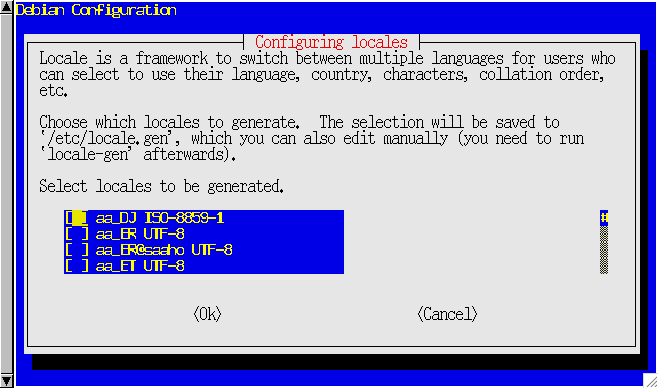
\includegraphics[width=1\hsize]{image200609/debconf-en.png}\\
これに対して日本語のロケールでは次のようになります。\\
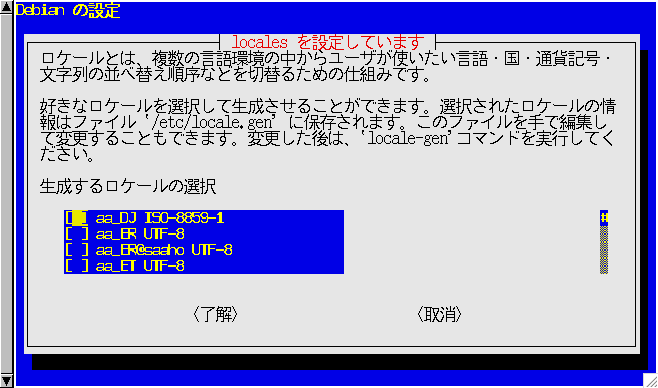
\includegraphics[width=1\hsize]{image200609/debconf-ja.png}\\
このようにロケールに応じた質問を提供するのがdebconf-poです。

このdebconfの質問自体は、次のように、パッケージ作者によって、
ソースパッケージのdebianディレクトリの下の
バイナリパッケージ用templatesファイルに英語で書かれています。\\
\begin{commandline}
Template: locales/locales_to_be_generated
Type: multiselect
Choices: ${locales}
_Description: Select locales to be generated.
 Locale is a framework to switch between multiple languages for users who can
 select to use their language, country, characters, collation order, etc.
 .
 Choose which locales to generate.  The selection will be saved to
 `/etc/locale.gen', which you can also edit manually (you need to run
 `locale-gen' afterwards).

Template: locales/default_environment_locale
Type: select
_Choices: None, ${locales}
Default: None
_Description: Which locale should be the default in the system environment?
 Many packages in Debian use locales to display text in the correct
 language for users. You can change the default locale if you're not
 a native English speaker.
 These choices are based on which locales you have chosen to generate.
 .
 Note: This will select the language for your whole system. If you're
 running a multi-user system where not all of your users speak the language
 of your choice, then they will run into difficulties and you might want
 not to set a default locale.

\end{commandline}

オリジナルは英語ですが、非英語圏のユーザにとっては、
自分の母語で質問されるほうがよいでしょう。
そこで、localizeされたdebconf質問をユーザが利用できるようにするのが、
このdebconf-poです。

\subsubsection{作業方法}

作業を開始する前に、
まずは\ref{subsubsec:debconf-po-check}で述べる翻訳状況調整ページで
既に翻訳作業が行われていないか確認するとよいでしょう。
その上で翻訳対象とするパッケージを決めたら、
\url{http://www.debian.org/intl/l10n/po-debconf/pot}からそのファイルの
templates.potファイルをダウンロードします。
もちろん、ソースパッケージを手に入れ、
目的のバイナリパッケージのtemplatesファイルに対して
\texttt{po-debconf}パッケージの\texttt{debconf-gettextize}コマンドを
実行し、templates.potを生成してもかまいません。

templates.potファイルを取得したら、
名前をja.poに変更した上で翻訳しましょう。

翻訳を終えたら、該当パッケージに対して、severityを「wishlist」、tagsを「l10n,
patch」としてバグ報告しましょう。
ただ、慣れていないうちはDebian JPのdebian-docメーリングリストで
査読してもらうことを強くお勧めします。

% FIXME: 余裕があったらもっと書く!!

\subsubsection{翻訳状況の確認}
\label{subsubsec:debconf-po-check}

debconf-poについては、翻訳状況に関する情報が以下のページで得られます。
\begin{itemize}
 \item debconf-poファイル翻訳のページ (%
       \url{http://www.debian.org/international/l10n/po-debconf/})
       \begin{itemize}
	\item 日本語の翻訳状況:
	      \url{http://www.debian.org/international/l10n/po-debconf/ja}
	\item 言語ごとの翻訳ランキング:
	      \url{http://www.debian.org/international/l10n/po-debconf/rank}
       \end{itemize}
 \item 武藤健志さんが提供するdebconf-po日本語翻訳作業調整ページ (%
	    \url{http://kmuto.jp/debian/po-trans/})
       各パッケージのdebconf-poの翻訳状況および最終訳者の情報を
       得ることができます。
\end{itemize}

\subsection{ウェブページ関連}

\subsubsection{Debianウェブページの仕組み}

DebianのウェブページはWMLというファイル形式を利用しています。
WMLとはウェブサイトメタ言語 (web site meta language) のことで、
Debianでは\texttt{wml}パッケージとして提供されています。
ここでは詳しくは述べませんが、
翻訳が原文に追従できているかの確認などがこのWMLの機構を用いて
行われている、ということだけ書いておきます。

次の例は、
\url{http://www.debian.org/News/weekly/2006/35/index}のソースとなってい
る、\texttt{cvs.debian.org}の\texttt{webwml}モジュール\footnote{%
\url{http://cvs.debian.org/?root=webwml}}の、
\texttt{webwml/japanese/News/weekly/2006/35/index.wml}です。\\
\begin{commandline}
#use wml::debian::weeklynews::header PUBDATE="2006-08-29"
 #SUMMARY="Firmware, FrOSCon, Events, Cuba, Translations, GIT, Sarge,
 #Etch" 
#use wml::debian::translation-check translation="1.8"

<p>Welcome to this year's 35th issue of DWN, the weekly newsletter for the
Debian community.  Bug squashing parties have been announced for September 8th
to 10th in <a
href="http://lists.debian.org/debian-devel-announce/2006/08/msg00012.html">\
Vienna</a> and for September 15th to 17th in <a
href="http://lists.debian.org/debian-devel-announce/2006/08/msg00013.html">\
J&uuml;lich</a>, Germany.  OSDir has taken <a
href="http://shots.osdir.com/slideshows/slideshow.php?release=724&amp;slide=2">\
Debian installer</a>.  Petr Stehlik <a
href="http://lists.debian.org/debian-68k/2006/08/msg00234.html">reported</a>
that the installation of <a href="$(HOME)/releases/sarge/">sarge</a> and <a
href="$(HOME)/releases/etch/">etch</a> worked flawlessly in the recently <a
href="http://lists.debian.org/debian-68k/2006/08/msg00226.html">fixed</a>
version of <a href="http://packages.debian.org/aranym">ARAnyM</a>, a 32bit
Atari ST/TT/Falcon virtual machine.</p>

[snip]

#use wml::debian::weeklynews::footer editor="Sebastian Feltel, Mohammed
 Adn&egrave;ne Trojette, Tobias Toedter, Martin 'Joey' Schulze" 
\end{commandline}

このうち\verb|#|で始まる行がWMLの命令です。
例えば、\\
\begin{commandline}
#use wml::debian::translation-check translation="1.8"
\end{commandline}

という行は、原文 (\texttt{webwml/english/News/weekly/2006/35/index.wml})
のr1.8に基づいているという意味です。

\subsubsection{作業方法}

翻訳作業を開始するには、目的のページのWMLファイルを入手する必要があります。
CVSを使い慣れている場合は、
コマンドラインから日本語のツリー (\texttt{webwml/japanese}) と
英語のツリー (\texttt{webwml/english}) をチェックアウトすると
よいでしょう。
CVSを使い慣れていない場合は\url{http://cvs.debian.org/?root=webwml}から
リポジトリビューアViewCVSを使って英語または日本語の目的のファイルを
ダウンロードしましょう。
ただし、この方法では後述するlatin-1文字の置換作業ができないため、
ページ内にlatin-1文字が含まれていた場合には自分で何とかして
対処しなければなりません。
したがって、こちらはあまりお勧めしません。

新規翻訳の場合、英語のファイルを取得したら、
まずはそれを日本語訳用に変換しなければなりません。
それには\texttt{webwml/copypage.pl}を用いて次のように実行します。\\
\begin{commandline}
nori1[6:12]%  DWWW_LANG=japanese ./copypage.pl english/News/weekly/2006/37/index.wml
Unable to open language.conf. Using environment variables...
Processing english/News/weekly/2006/37/index.wml...
Destination directory japanese/News/weekly/2006/37/ does not exist,
Copied News/weekly/2006/37/index.wml, remember to edit japanese/News/weekly/2006/37/index.wml
\end{commandline}

こうすると、オリジナルのファイルのリビジョンを元にして、
前述の \texttt{wml::debian::translation-check translation} の値が適切に
設定されます。
また、latin-1でエンコードされた文字列があっても適切な文字実体参照に
置換され、
日本語の文字と欧米の文字が共存できるようになります。
あとは自由に翻訳してください。

新規翻訳ではなく、翻訳が古くなったページの更新であれば、
英語のページを日本語用にコピーする必要はありません。
\texttt{wml::debian::translation-check translation} の値を適切に設定し、
原文の差分を見ながら翻訳を更新しましょう。

翻訳の際のルールについては、
\url{http://www.debian.or.jp/devel/www/WebTranslation.html}を参照すると
よいでしょう。
また、
ウェブページはMozilla FirefoxのようなGUIのウェブブラウザでもw3mのような
テキストブラウザでも美しく見えてほしいので、
改行位置には気をつけることになっています。
\url{http://lists.debian.or.jp/debian-www/200408/msg00046.html}や
\url{http://lists.debian.or.jp/debian-www/200609/msg00102.html}などを
参考にしてください。

翻訳が終わったら、
Debian JPのdebian-wwwメーリングリストに査読・コミット依頼を出します。
現在はコミットは主に今井伸広さんがしてくださっています。

% FIXME: 余裕があったらもっと書く!!

\subsubsection{翻訳状況の確認}
\label{subsubsec:www-check}

ウェブページについては、翻訳状況に関する情報が以下のページで得られます。
\begin{description}
 \item[ウェブサイト翻訳状況
	    (\url{http://www.debian.org/devel/website/stats/})] 
	    言語ごとの翻訳状況の統計が載っています。
 \item[日本語のウェブサイト翻訳状況
	    (\url{http://www.debian.org/devel/website/stats/ja.html})] 
	    日本語の各ファイルの翻訳状況がわかります。
\end{description}

\subsection{The Debian Description Translation Project (DDTP)}

\subsubsection{DDTPとは}

Debian Description Translation Project (DDTP) とは、
現在すべて英語で提供されているDebianパッケージ説明文 (Description) に
翻訳を提供し、
それらの翻訳情報が使えるインフラを整えようというプロジェクトです。
\url{http://ddtp.debian.net/}がプロジェクトのウェブサイトです。

おそらく皆さん御存知でしょうが、
パッケージ説明文とはパッケージ付随情報の一つで、
パッケージの内容を説明するとともに、
\texttt{aptitude search}などでパッケージを検索する際に便利になるよう
提供されています。
以下は、sargeで\texttt{aptitude}パッケージの情報を表示させたときの
様子で、「詳細:」で始まる行\footnote{aptitude
0.4.2以降では「説明文:」という訳語に変わっています。}以降が
パッケージ説明文です。\\
\begin{commandline}
nori1[12:04]%  aptitude show aptitude            whale:~/svnwc/deb/skkdic/trunk
パッケージ: aptitude
ステータス: インストール済み
自動的にインストールされる: no
バージョン: 0.2.15.9-6bpo3
優先度: 任意
分類: admin
保守担当者: Daniel Burrows <dburrows@debian.org>
展開サイズ: 5288k
依存: libapt-pkg-libc6.3-5-3.11, libc6 (>= 2.3.2.ds1-21), libgcc1 (>=
      1:3.4.1-3), libncurses5 (>= 5.4-1), libsigc++-1.2-5c102, libstdc++5 (>=
      1:3.3.4-1)
提案: aptitude-doc-en | aptitude-doc
詳細: terminal-based apt frontend
 aptitude is a terminal-based apt frontend with a number of useful features,
 including: a mutt-like syntax for matching packages in a flexible manner,
 dselect-like persistence of user actions, the ability to retrieve and display
 the Debian changelog of most packages, and extreme flexibility and
 customization.

 aptitude is also Y2K-compliant, non-fattening, naturally cleansing, and
 housebroken.

\end{commandline}

このパッケージ説明文のエントリ自体は、次のように、パッケージ作者によって、
ソースパッケージのdebian/controlファイルに英語で書かれています。\\
\begin{commandline}
[snip]
Description: terminal-based apt frontend
 aptitude is a terminal-based apt frontend with a number of useful
 features, including: a mutt-like syntax for matching packages in a
 flexible manner, dselect-like persistence of user actions, the
 ability to retrieve and display the Debian changelog of most
 packages, and extreme flexibility and customization.
 .
 aptitude is also Y2K-compliant, non-fattening, naturally cleansing,
 and housebroken.
[snip]
\end{commandline}

説明文は、\verb|Description:|と同じ行に書かれるshort descriptionと、
その後のlong descriptionに分かれます。

オリジナルは英語ですが、非英語圏のユーザにとっては、
自分の母語でパッケージ説明文を読めるほうがよいでしょう。
そこで、localizeされたパッケージ説明文をユーザが利用できるようにする
ことを目的として作られたのがこのDDTPというプロジェクトです。

このプロジェクトは数年前から存在しており、
日本語についても日本語チームコーディネータの田村一平さんなどが
積極的に作業を進め、
一時は翻訳率でトップになったこともありました\footnote{%
\url{http://d.hatena.ne.jp/denson/20050315/p2}}が、
Debianのホストの問題で暫く停止していました。
完全にではありませんが、
最近ようやく復活の兆しが見え始めました\footnote{%
\url{http://www.debian.org/News/weekly/2006/31/}や
\url{http://www.debian.org/News/weekly/2006/35/}に関連記事があります。
\url{http://lists.debian.org/debian-devel/2006/07/msg01323.html}から
始まる ``Translated packages descriptions progress'' というスレッドも
盛り上がっていました。}。
最近は以下のような状況です。
\begin{itemize}
 \item Debian本家のウェブサイトにもDDTPのページ
       \footnote{\url{http://www.debian.org/international/l10n/ddtp}}が
       作られた。
 \item プロジェクトウェブサイトが復活し、翻訳状況を見られるようになった。
 \item メールインタフェース (後述) が復活した。
 \item ウェブインタフェース (後述) が作られた。
\end{itemize}

\subsubsection{作業方法}

DDTPの作業方法については、
Debian JPのサイトに日本語の説明があります\footnote{%
\url{http://www.debian.or.jp/devel/doc/Description-ja.html}}。
ただしこれは復活前のもので情報がやや古くなっているので、
最近作られたDebian本家のウェブサイトのDDTPのページ\footnote{%
\url{http://www.debian.org/international/l10n/ddtp}}を参照するのが
よいでしょう。
このページは本資料執筆現在は英語でしか利用できないので、
ここでは本家の説明に基づいて、簡単に説明します\footnote{%
本家のDDTPのページは近々日本語で利用可能になる予定です。
今後はDebian JPのページではなくそちらのページをメインの日本語情報として
参照するとよいでしょう。}。

\subsubsubsection{メールインタフェース}

DDTPは、誰でも気軽に作業できるよう、
非常に簡単なインタフェースを通じて作業できるようになっています。
現在Debianパッケージ数は15000を超えており、
debconfとは異なりパッケージ説明文はすべてのパッケージに含まれているので、
それらをすべてlocalizeしようという目的をもつこのプロジェクトは、
とても壮大で大量のマンパワーを必要とするからです。
新しいパッケージでパッケージ説明文が改良されることがあるので、
それらの変化にも追従できなければいけません。

公式インタフェースはメールで、
それ以外にもウェブインタフェースが開発されています。

メールインタフェースを使うには、
次のような件名 (Subject) で\texttt{pdesc@ddtp.debian.net}にメールを
送ってください。\\
\begin{commandline}
GET n lang
\end{commandline}

\texttt{n}はパッケージ説明文の数で、9以下の数値を指定してください。
\texttt{lang}は言語コードで、日本語では\texttt{ja}です。
\texttt{lang}の後ろにドット (\texttt{.}) に繋げてエンコーディングを
指定することも可能です。

メールを送ると、
指定された数だけパッケージ説明文が添付されたメールが返信されます。
これらのパッケージ説明文はしばらくの時間ロックされ、
メールで取り寄せた人のみが作業できるようになるので、
安心してゆっくり作業しましょう。
各添付ファイルは次のような形式になっているので、
パッケージ説明文中の\texttt{<trans>}と記された部分を翻訳してください。\\
\begin{commandline}

# Source: aolserver4-nsopenssl
# Package(s): aolserver4-nsopenssl
# Prioritize: 45
# This Description is active
# This Description is owned
Description: AOLserver 4 module: module for SSL mode.
 This module adds SSL capabilities to aolserver, and gives Tcl scripts
 an API to access openssl functions.
 .
 This is currently a beta release! Use at your own risk.
Description-ja.euc-jp: <trans>
 <trans>
 .
 <trans>
#
# other Descriptions of the aolserver4-nsopenssl package with a translation in ja:
# 
\end{commandline}

翻訳するのは、\texttt{<trans>}だけです。
英語のパッケージ説明文は変更しないでください\footnote{誤りを発見したら
そのパッケージのバグとしてBTSにバグ報告してください。}。
また、ドットだけの行も段落のセパレータとして重要なので、
変更を加えないでください。
ただし、
上の例ではshort descriptionとlong descriptionの各段落の内容がすべて
\texttt{<trans>}となっていますが、
一部の段落に既に翻訳が入っている場合もあります。
それは、他のパッケージに同じ段落が含まれておりそれが翻訳済みの場合です。
これらは修正してもかまいません。

エンコーディングは正しいものを用いるよう注意してください。
例えば、
\texttt{GET 1 ja}という件名でパッケージ説明文を取り寄せると、
\texttt{GET 1 ja.euc-jp noguide}という件名のメールが返ってきます。
これは、日本語のデフォルトエンコーディングがEUC-JPとなっているからです。
この場合、翻訳したファイルのエンコーディングはEUC-JPとし、
メールで送る際にもISO-2022-JPで送ってしまわないよう気をつけてください。
ただし、上の例の翻訳部のフィールドが\texttt{Description-ja.euc-jp}と
なっていることからもわかるように、
エンコーディング指定は変更可能です。
UTF-8がいいというのであれば、
フィールド名を\texttt{Description-ja.UTF-8}として翻訳文字列をUTF-8で
記入してください。

翻訳を終えたらファイルを\texttt{pdesc@ddtp.debian.net}に送り返します。
翻訳文はbase64エンコードするとよいでしょう。
中野武雄さん作のddts-send\footnote{%
\url{http://surf.ap.seikei.ac.jp/~nakano/linux/ddts-send.ja.html}}や
\texttt{ddtc}パッケージ\footnote{%
\url{http://packages.debian.org/ddtc}}などのヘルパーも利用可能です。

\subsubsubsection{ウェブインタフェース}

Martijn van Oosterhoutさんが作成したウェブインタフェースはDDTSSと呼ばれ、
\url{http://kleptog.org/cgi-bin/ddtss2-cgi/xx}にあります。
翻訳と査読・校正の作業をウェブで簡単に行えるようになっています。

% FIXME: もっと書く!!

\subsubsection{翻訳状況の確認}

DDTPでは、翻訳状況の確認は以下のページでできます。

\begin{description}
 \item[プロジェクトウェブサイト (\url{http://ddtp.debian.net/})]
	    トップページには言語ごとの翻訳状況の統計が載っています。
	    パッケージごとに各言語への翻訳状況を表示することも可能です。
\end{description}

\subsubsection{翻訳内容の取得}

DDTPによるパッケージ説明文の翻訳は、Debianのミラーの
\url{http://ftp.jp.debian.org/debian/dists/sid/main/i18n/}などから
取得可能です。
例えば日本語なら、上記のディレクトリのTranslation-ja.gzや
Translation-ja.bz2が利用できます。

\subsection{おわりに}

本節では、国際化の一環として重要な翻訳について、
作業方法および各種情報を取得できるページをざっと説明しました。
翻訳は非常に手間がかかる作業で、膨大なマンパワーを必要とします。
Debianではあなたの参加を心待ちにしています。

\subsection{参考文献}

以下のページも参考にしてください。

\begin{itemize}
 \item 武藤健志さんのblogの『Debianドキュメント翻訳手続き』:
       \url{http://kmuto.jp/d/index.cgi/debian/debian-doc-procedure.htm}
\end{itemize}

%% 小林さんここまで

\dancersection{dpkg, apt のプロファイリング}{上川}
\label{sec:dancerjapt}

apt や dpkg のどの部分が一番遅いのか、実際にプロファイリングしてみます。
この例をケーススタディーとして、一般的にどういう作業をすればパフォーマンス
チューニングが必要な部分を抽出できるのか、をあきらかにしてみましょう。

\subsection{oprofile のインストールと設定方法}

Debianのデフォルトのカーネルはoprofileをサポートしています
\footnote{i386, amd64 などのアーキテクチャ以外での利用は現時点では難し
い可能性があるので確認してください。}。もし、自分でコンパイルしていたり
して oprofile サポートを追加していない場合は、カーネルを oprofile サポー
ト付きでコンパイルしなおします。オプションは \texttt{CONFIG\_OPROFILE}
です。メニューでは

\texttt{Intrumentation support : Profiling Support :
Oprofile system profiling (experimental)}\footnote{2.6.18-rc1 現在}

にあります。

カーネルがサポートしている場合、oprofileを利用するのに追加で必要なのは
\texttt{oprofile}パッケージです。
\texttt{apt-get install oprofile}でインストールしましょう。

カーネルのシンボルのプロファイリング\footnote{無い場合はカーネルの内部の
どこかで実行していることはわかるが、実際どの関数で時間がかかっているのか、
ということがわからない。}をするために、vmlinuxファイルが必要です。
カーネルを自分でコンパイルした場合には、ビルドしたディレクトリに
vmlinux ファイルがあります。 make-kpkg を利用してビルドしたのであれば、

\begin{commandline}
 /lib/modules/$(uname -r)/build
\end{commandline}

から適切にリンクがはられているはずです。探してみてください。
\footnote{oprofile メーリングリストには vmlinux ファイルよりは普及している System.map を利用するパッチ
というのも存在するので、それを適用してみるのもよいかもしれません。}

\subsection{oprofile が自分の利用しているCPUをサポートしていない場合}

残念ながら9月現在時点の Debian Package では、Intel core duo CPU 上では 
oprofile が動作しません。oprofile は認識できていない場合、\texttt{cpu\_type} 変数
が unset という値になります。カーネル側は \texttt{cpu\_type} として i386/core を
出力しているので、この時点でどうやらカーネル側のサポートは追加されている
らしいということがわかります。

\begin{commandline}
$ sudo opcontrol --init
cpu_type 'unset' is not valid
$ opcontrol --list-events
Unable to open cpu_type file for reading
Make sure you have done opcontrol --init
cpu_type 'unset' is not valid
$ cat /dev/oprofile/cpu_type
i386/core
$ uname -a
Linux coreduo 2.6.18-rc1dancer #2 SMP Sun Jul 9 09:57:01 JST 2006 i686 GNU/Linux
\end{commandline}

プロファイルを取得するという目的を考えると手段としてはいくつか考えられます。

\begin{itemize}
 \item プロファイルの仕組はあまりかわらないだろうと見込み、
       \texttt{arch/i386/oprofile/nmi\_int.c}の \texttt{ppro\_init} を修正、
       piiiとかに見せてしまう

 \item まじめにoprofileのユーザ空間アプリケーションを修正、core duo の
       仕様書を読み、対応を追加

 \item おそらくすでに修正されていることを見越して、oprofile の CVS レポ
       ジトリをみにいく       

 \item 実験することが目的なのでサポートされているCPUのマシンを準備する

\end{itemize}

今回はoprofileの開発メーリングリストを見たところ、5月の時点でだれかがパッ
チを書いているのを発見したので、それをとりこみます。
念のため、今後作業する人のためにBTSにも登録しました (\debianbug{380462})。

確認してみると、どうやら動作してくれていることがわかりました。ここで、当
面重要なのは、 \texttt{CPU\_CLK\_UNHALTED} でしょう。CPUサイクルがどの関数で消費
されているのかということをトラッキングできます。まずCPUの処理負荷がかかっ
ている部分を目視して、何か問題がないかを眺めてみて、何も問題なく、それな
りに問題が追求できにくくなった後に、L2キャッシュのイベントの発生度合とか
を確認していけばよいでしょう。

\begin{commandline}
$ sudo opcontrol --init
$ sudo opcontrol --list-events
oprofile: available events for CPU type "Core Solo / Duo"

See Intel Architecture Developer's Manual Volume 3, Appendix A and
Intel Architecture Optimization Reference Manual (730795-001)

CPU_CLK_UNHALTED: (counter: all)
        Unhalted clock cycles (min count: 6000)
        Unit masks (default 0x0)
        ----------
        0x00: Unhalted core cycles
        0x01: Unhalted bus cycles
        0x02: Unhalted bus cycles of this core while the other core is halted
INST_RETIRED: (counter: all)
        number of instructions retired (min count: 6000)
L2_RQSTS: (counter: all)
        number of L2 requests (min count: 6000)
        Unit masks (default 0xf)
        ----------
        0x08: (M)odified cache state
        0x04: (E)xclusive cache state
        0x02: (S)hared cache state
        0x01: (I)nvalid cache state
        0x0f: All cache states
        0x10: HW prefetched line only
        0x20: all prefetched line w/o regarding mask 0x10.

[省略]

\end{commandline}

\subsection{デバッグシンボルを収集する:dpkg と apt をコンパイルしなおす}

まず、デバッグ情報がすでにあるパッケージについては、インストールします。
今回では、大きいものとして、libc6-dbg パッケージがあるので、それはインス
トールします。プロファイルの結果、イメージが上位に出現するなどで、必要そ
うであれば、あとで他のライブラリなどについてもデバッグ情報のあるバージョ
ンを追加しましょう。

今回プロファイル対象の dpkg と apt はデフォルトではデバッグ情報がありませ
ん、プロファイル出力を確認しやすいように、デバッグシンボルを追加してコン
パイルしなおします。

\begin{commandline}
 $ debuild -e DEB_BUILD_OPTIONS=nostrip
\end{commandline}
%$

その後、インストールします。

まず、oprofileを実行するのを便利にするために、スクリプトを仕込みます。
入力されたコマンドを10回実行してそのプロファイルを取得するというものです。

\begin{commandline}
 read CMD
 sudo opcontrol --shutdown
 sudo opcontrol --reset
 sudo opcontrol --setup \
  --vmlinux=/lib/modules/$(uname -r)/build/vmlinux \
    --event=CPU_CLK_UNHALTED:180000:0:1:1 --separate=library
    sudo opcontrol --start
 for A in $(seq 1 10); do
   $CMD
 done
 opcontrol --dump && \
 opreport -l -p /lib/modules/$(uname -r)/kernel 2>/dev/null \
  | head -30
\end{commandline}

まず、デバッグ用のバイナリが正常に作成できているか簡単に確認します。まず、
apt-get update をループでまわしてみます。libapt-pkgのシンボルレベルで確
認できているので、デバッグシンボルが存在しているということがわかります。

\begin{commandline}
sudo apt-get update
[中略]
CPU: Core Solo / Duo, speed 1833 MHz (estimated)
Counted CPU_CLK_UNHALTED events (Unhalted clock cycles) with a unit mask of 0x00 (Unhalted core cycles) count 180000
samples  %        image name               app name                 symbol name
23823    46.3519  libapt-pkg-libc6.3-6.so.3.11.0 apt-get                  
SHA1Transform(unsigned int*, unsigned char const*)
12732    24.7724  libapt-pkg-libc6.3-6.so.3.11.0 apt-get
 MD5Transform(unsigned int*, unsigned int const*) 
4282      8.3314  processor.ko             processor                acpi_processor_idle
2584      5.0276  libc-2.3.6.so            apt-get                  (no symbols)
2012      3.9147  vmlinux                  vmlinux                  __copy_to_user_ll
503       0.9787  gpgv                     gpgv                     (no symbols)
222       0.4319  vmlinux                  vmlinux                  timer_interrupt
166       0.3230  libapt-pkg-libc6.3-6.so.3.11.0 apt-get
 MD5Summation::Add(unsigned char const*, unsigned long) 
160       0.3113  vmlinux                  vmlinux                  page_fault
158       0.3074  libapt-pkg-libc6.3-6.so.3.11.0 apt-get
 SHA1Summation::Add(unsigned char const*, unsigned long) 
140       0.2724  libstdc++.so.6.0.8       apt-get                  (no symbols)
134       0.2607  vmlinux                  vmlinux                  find_get_page
125       0.2432  ld-2.3.6.so              http                     do_lookup_x
123       0.2393  vmlinux                  vmlinux                  sysenter_past_esp
95        0.1848  libapt-pkg-libc6.3-6.so.3.11.0 apt-get                  .plt
94        0.1829  ld-2.3.6.so              gpgv                     do_lookup_x
89        0.1732  libc-2.3.6.so            http                     (no symbols)
89        0.1732  vmlinux                  vmlinux                  do_generic_mapping_read
88        0.1712  ld-2.3.6.so              file                     do_lookup_x
87        0.1693  vmlinux                  vmlinux                  memcpy
72        0.1401  ld-2.3.6.so              http                     strcmp
69        0.1343  vmlinux                  vmlinux                  _spin_lock
65        0.1265  vmlinux                  vmlinux                  vfs_read
64        0.1245  ld-2.3.6.so              gpgv                     _dl_elf_hash
62        0.1206  vmlinux                  vmlinux                  __handle_mm_fault
60        0.1167  ld-2.3.6.so              http                     _dl_elf_hash
58        0.1128  oprofiled                oprofiled                (no symbols)
\end{commandline}

dpkgについてもプロファイリングしてみます。\footnote{ここで問題が出ました。
libc6 の dbg パッケージの情報を oprofile が処理できていないようです。
straceで解析してみましたが、ファイルをひらくところまでは何かできているよ
うです。これは別途バグ報告してみます (\debianbug{385704})。}

\begin{commandline}
sudo dpkg -i ../dselect_1.13.22_i386.deb
[中略]
CPU: Core Solo / Duo, speed 1833 MHz (estimated)
Counted CPU_CLK_UNHALTED events (Unhalted clock cycles) with a unit mask of 0x00 (Unhalted core cycles) count 180000
samples  %        image name               app name                 symbol name
41009    32.6009  libc-2.3.6.so            dpkg                     (no symbols)
27485    21.8497  processor.ko             processor                acpi_processor_idle
14863    11.8156  dpkg                     dpkg                     parsedb
4845      3.8516  dpkg                     dpkg                     findnamenode
2691      2.1393  dpkg                     dpkg                     findpackage
1994      1.5852  dpkg                     dpkg                     f_dependency
1742      1.3848  vmlinux                  vmlinux                  get_page_from_freelist
1660      1.3196  dpkg-deb                 dpkg-deb                 inflate_fast
1552      1.2338  dpkg                     dpkg                     iterpkgnext
1520      1.2084  dpkg                     dpkg                     .plt
1500      1.1925  dpkg                     dpkg                     varbufaddbuf
1192      0.9476  dpkg                     dpkg                     filesdbinit
1080      0.8586  dpkg                     dpkg                     w_dependency
1001      0.7958  dpkg                     dpkg                     varbufdependency
988       0.7854  dpkg                     dpkg                     nfmalloc
884       0.7028  dpkg                     dpkg                     illegal_packagename
849       0.6749  vmlinux                  vmlinux                  page_fault
802       0.6376  vmlinux                  vmlinux                  __copy_from_user_ll_nocache_nozero
687       0.5461  dpkg                     dpkg                     ensure_packagefiles_available
633       0.5032  dpkg                     dpkg                     varbufaddc
568       0.4515  dpkg                     dpkg                     f_filecharf
516       0.4102  vmlinux                  vmlinux                  __copy_to_user_ll
473       0.3760  dpkg                     dpkg                     copy_dependency_links
458       0.3641  dpkg                     dpkg                     parseversion
427       0.3395  dpkg                     dpkg                     ensure_package_clientdata
406       0.3228  dpkg                     dpkg                     nfstrsave
384       0.3053  dpkg                     dpkg                     varbufrecord
\end{commandline}

パッケージをインストールして削除する、というループを回してみましょう。
\texttt{apt-listbugs}と\texttt{apt-listchanges}が含まれており、ruby と
pythonの処理負荷が高いことがわかります。また、libc6のなかで何か重たい処
理をしているのがわかります。

\begin{commandline}
 sudo apt-get install -y dsh; sudo apt-get remove -y libdshconfig1
[中略]
Counted CPU_CLK_UNHALTED events (Unhalted clock cycles) with a unit mask of 0x00 (Unhalted core cycles) count 180000
samples  %        image name               app name                 symbol name
195383   24.3783  processor                processor                (no symbols)
114285   14.2595  libc-2.3.6.so            dpkg                     (no symbols)
67157     8.3793  libruby1.8.so.1.8.4      ruby1.8                  (no symbols)
48893     6.1005  libc-2.3.6.so            dpkg-query               (no symbols)
41537     5.1826  dpkg                     dpkg                     parsedb
30685     3.8286  perl                     perl                     (no symbols)
28353     3.5377  dpkg-query               dpkg-query               parsedb
26135     3.2609  python2.4                python2.4                (no symbols)
13951     1.7407  libc-2.3.6.so            ruby1.8                  (no symbols)
10023     1.2506  libc-2.3.6.so            apt-get                  (no symbols)
9138      1.1402  dpkg                     dpkg                     findnamenode
7914      0.9874  vmlinux                  vmlinux                  get_page_from_freelist
7656      0.9553  dpkg                     dpkg                     findpackage
5963      0.7440  vmlinux                  vmlinux                  read_hpet
5777      0.7208  libc-2.3.6.so            perl                     (no symbols)
5465      0.6819  dpkg                     dpkg                     f_dependency
5108      0.6373  dpkg-query               dpkg-query               findpackage
4525      0.5646  dpkg                     dpkg                     filesdbinit
4452      0.5555  libapt-pkg-libc6.3-6.so.3.11.0 apt-get
 pkgDepCache::CheckDep(pkgCache::DepIterator, int,
 pkgCache::PkgIterator&) 
4237      0.5287  vmlinux                  vmlinux                  page_fault
4182      0.5218  dpkg                     dpkg                     .plt
4101      0.5117  dpkg                     dpkg                     varbufaddbuf
3874      0.4834  dpkg-query               dpkg-query               f_dependency
3744      0.4671  dpkg                     dpkg                     iterpkgnext
3645      0.4548  libstdc++.so.6.0.8       apt-get                  (no symbols)
3287      0.4101  libapt-pkg-libc6.3-6.so.3.11.0 apt-get
 pkgProblemResolver::MakeScores() 
3277      0.4089  vmlinux                  vmlinux                  delay_tsc
\end{commandline}

\subsection{テスト環境の作成}

テスト用の環境を作成します。今回はchroot 内部で大量の apt-get update,
apt-get install と apt-get remove をループで実行してベンチマークをとって
みましょう。

dpkgとaptを変更すると最悪システムが動作しなくなるため、テスト用に環境を
準備することは大切です。

chroot 内部では、chroot外部のファイルにアクセスすることができません。そ
のため、bind-mount を行い、外部のファイルを中に見せます。中で必要になる
ファイルとしては、apt/dpkgのデバッグ版、oprofileの修正版パッケージ(あれ
ば)、そして実行中のLinux kernel に対応するvmlinux ファイルです。

\begin{commandline}
 $ sudo cowbuilder --login --bindmount $(pwd)
 # apt-get install gnupg
 # apt-get update
 # apt-get install oprofile libc6-dbg
 # dpkg -i (bind-moumtしたところにおいた事前準備した apt/dpkg/oprofile)
 # apt-get -y install gnome; apt-get -y remove libglib2.0-0
 # unset LD_PRELOAD
 # unset COWDANCER_ILISTFILE
 # mount -t oprofilefs nodev /dev/oprofile >/dev/null
\end{commandline}

chroot で調べてみると、perlが一番重たい処理をしているということがわかり
ました。こりゃチューニングしにくいですね。依存関係の解決などの処理に時間
がかかっているかと仮説をたてていたのですが、特に露骨に目立って負荷の高い
関数というのは見付けることはできませんでした。

\begin{commandline}
apt-get install -y dsh; apt-get remove -y libdshconfig1
[中略]
CPU: Core Solo / Duo, speed 1833 MHz (estimated)
Counted CPU_CLK_UNHALTED events (Unhalted clock cycles) with a unit mask of 0x00 (Unhalted core cycles) count 180000
samples  %        image name               app name                 symbol name
51258    32.2132  processor                processor                (no symbols)
7929      4.9830  libc-2.3.6.so            apt-get                  (no symbols)
7321      4.6009  libc-2.3.6.so            dpkg                     (no symbols)
5239      3.2925  vmlinux                  vmlinux                  read_hpet
4377      2.7507  libc-2.3.6.so            perl                     (no symbols)
4282      2.6910  libapt-pkg-libc6.3-6.so.3.11.0 apt-get
 pkgDepCache::CheckDep(pkgCache::DepIterator, int,
 pkgCache::PkgIterator&) 
2888      1.8150  libstdc++.so.6.0.8       apt-get                  (no symbols)
2570      1.6151  libapt-pkg-libc6.3-6.so.3.11.0 apt-get
 debVersioningSystem::CmpFragment(char const*, char const*, char const*,
 char const*) 
2548      1.6013  libapt-pkg-libc6.3-6.so.3.11.0 apt-get
 pkgProblemResolver::MakeScores() 
2045      1.2852  dpkg                     dpkg                     parsedb
2019      1.2688  libapt-pkg-libc6.3-6.so.3.11.0 apt-get
 debVersioningSystem::DoCmpVersion(char const*, char const*, char
 const*, char const*) 
1722      1.0822  libapt-pkg-libc6.3-6.so.3.11.0 apt-get
 pkgDepCache::Update(OpProgress*) 
1571      0.9873  dpkg                     dpkg                     findnamenode
1558      0.9791  perl                     perl                     Perl_sv_gets
1461      0.9182  perl                     perl                     Perl_yyparse
1408      0.8849  libapt-pkg-libc6.3-6.so.3.11.0 apt-get
 debVersioningSystem::CheckDep(char const*, int, char const*) 
1222      0.7680  vmlinux                  vmlinux                  __copy_to_user_ll
1181      0.7422  vmlinux                  vmlinux                  get_page_from_freelist
1129      0.7095  perl                     perl                     S_hv_fetch_common
1055      0.6630  perl                     perl                     Perl_yylex
1054      0.6624  ldconfig                 ldconfig                 (no symbols)
1051      0.6605  libapt-pkg-libc6.3-6.so.3.11.0 apt-get
 OpProgress::CheckChange(float) 
1050      0.6599  vmlinux                  vmlinux                  page_fault
911       0.5725  libapt-pkg-libc6.3-6.so.3.11.0 apt-get
 pkgPolicy::GetCandidateVer(pkgCache::PkgIterator) 
816       0.5128  dpkg                     dpkg                     filesdbinit
815       0.5122  libapt-pkg-libc6.3-6.so.3.11.0 apt-get
 pkgDepCache::DependencyState(pkgCache::DepIterator&) 
793       0.4984  libapt-pkg-libc6.3-6.so.3.11.0 apt-get                  .plt
\end{commandline}

まず、opreportの結果を確認します。カーネル空間で16\%, apt-get で 10\%,
perl で 7\% であることがわかります。ここで重要なのは、この時点で dpkg 
をチューニングしても大して結果に反映しなさそうだということが明確になった
ことです。

\begin{commandline}
# opreport 
CPU: Core Solo / Duo, speed 1833 MHz (estimated)
Counted CPU_CLK_UNHALTED events (Unhalted clock cycles) with a unit mask of 0x00 (Unhalted core cycles) count 180000
CPU_CLK_UNHALT...|
  samples|      %|
------------------
   182440 51.3356 processor
    59664 16.7885 vmlinux
    38517 10.8380 apt-get
        CPU_CLK_UNHALT...|
          samples|      %|
        ------------------
            25578 66.4070 libapt-pkg-libc6.3-6.so.3.11.0
             7929 20.5857 libc-2.3.6.so
             2888  7.4980 libstdc++.so.6.0.8
             1701  4.4162 apt-get
              381  0.9892 ld-2.3.6.so
               12  0.0312 anon (tgid:31689 range:0xb7f47000-0xb7f48000)
               11  0.0286 anon (tgid:31917 range:0xb7f49000-0xb7f4a000)
                9  0.0234 anon (tgid:31841 range:0xb7fcb000-0xb7fcc000)
                8  0.0208 anon (tgid:31765 range:0xb7f9d000-0xb7f9e000)
    27091  7.6230 perl
        CPU_CLK_UNHALT...|
          samples|      %|
        ------------------
            22216 82.0051 perl
             4377 16.1567 libc-2.3.6.so
              273  1.0077 libpthread-2.3.6.so
              214  0.7899 ld-2.3.6.so
                3  0.0111 libnss_compat-2.3.6.so
                2  0.0074 libdl-2.3.6.so
                2  0.0074 Fcntl.so
                1  0.0037 libnss_files-2.3.6.so
                1  0.0037 libnss_nis-2.3.6.so
                1  0.0037 IO.so
                1  0.0037 gettext.so
    23916  6.7296 opreport
        CPU_CLK_UNHALT...|
          samples|      %|
        ------------------
            14091 58.9187 opreport
             5445 22.7672 libc-2.3.6.so
             4119 17.2228 libstdc++.so.6.0.8
              257  1.0746 ld-2.3.6.so
                3  0.0125 libgcc_s.so.1
                1  0.0042 libpopt.so.0.0.0
    16010  4.5049 dpkg
        CPU_CLK_UNHALT...|
          samples|      %|
        ------------------
             8611 53.7851 dpkg
             7321 45.7277 libc-2.3.6.so
               74  0.4622 ld-2.3.6.so
 
\end{commandline}

この後試行錯誤して apt-get update の処理についてはチューニングできそうだ、
ということがわかったのですが、それはまた別の機会に。

\subsection{まとめ}

この文章では Debian で oprofile を利用してボトルネックを検出する作業をす
るための手順についてまとめました。

\subsection{参考文献}

\begin{itemize}
 \item rpmのプロファイリング \url{https://www.redhat.com/magazine/012oct05/features/oprofile/}
\end{itemize}

\dancersection{aptを最適化してみる}{上川}

前回までで、oprofile を利用して aptのプロファイリングをしてみました。そ
れでは、実際にどういう考え方で高速化を検討するか、を考えてみましょう。

\subsection*{最適化の必要な部分の解析}

プロファイル結果を利用して、解析します。

\texttt{apt-get update}の結果を確認したところ、下記のようになるということ
がわかりました。どうも、\texttt{SHA1Transform} と \texttt{MD5Transform} という関数の負荷
が高いようです。

\begin{commandline}
sudo apt-get update
[中略]
CPU: Core Solo / Duo, speed 1833 MHz (estimated)
Counted CPU_CLK_UNHALTED events (Unhalted clock cycles) with a unit mask of 0x00 (Unhalted core cycles) count 180000
samples  %        image name               app name                 symbol name
23823    46.3519  libapt-pkg-libc6.3-6.so.3.11.0 apt-get                  
SHA1Transform(unsigned int*, unsigned char const*)
12732    24.7724  libapt-pkg-libc6.3-6.so.3.11.0 apt-get
 MD5Transform(unsigned int*, unsigned int const*) 
4282      8.3314  processor.ko             processor                acpi_processor_idle
2584      5.0276  libc-2.3.6.so            apt-get                  (no symbols)
2012      3.9147  vmlinux                  vmlinux                  __copy_to_user_ll
503       0.9787  gpgv                     gpgv                     (no symbols)
222       0.4319  vmlinux                  vmlinux                  timer_interrupt
166       0.3230  libapt-pkg-libc6.3-6.so.3.11.0 apt-get
 MD5Summation::Add(unsigned char const*, unsigned long) 
\end{commandline}

\subsection*{最適化方法の検討}

プロファイル結果解析をうけて適用できる最適化方法を検討します。

\texttt{apt-pkg/contrib/sha1.cc}, \texttt{apt-pkg/contrib/md5.cc} を見る
と md5 については、 dpkg の実装を、 sha1についてはどこからか拾ってきた実
装を利用しており、 C++ で書かれた汎用のコードを利用しているということが
わかります。仮説として、アッセンブリでばりばりにチューニングした実装を利
用すれば高速になるのではないか、と考えてみます。

GPL 互換の既存の sha1 と md5 の高速な実装を探してみます。

代表的な GPL 互換の実装である GNUTLS に含まれている sha1 / md5 の実装は、 
\texttt{gl/sha1.c}, \texttt{gl/md5.c} にあます。確認したところ、特に高速
化されていないようです。

そこで、 git のソースを見てみます。ppc と arm 用の最適化されている sha1 
の実装が含まれていますが、 i386 用はないようです。

予備試験をしてみます。600MB程度の iso ファイルの sha1 をとるのに、
mozilla 実装と openssl 実装でどらくらい違うのかを比較してみました。
mozilla 実装で 14 秒程度、openssl 実装で 12 秒程度です。

ここまでで、既存の実装を応用する限りにおいて、試験環境において劇
的に高速化できる方策は無いということがわかりました。残念。


\dancersection{Jamon, tinto vino, por favor. --スペインExtremadura州Debian i18n会議報告}{武藤 健志 \texttt{<kmuto@debian.org>}}
\label{sec:extremadura}

去る2006年9月7日〜9月9日の期間、スペインExtremadura州Casar de C\'{a}ceres(図\ref{fig:casar})において開催された「第1回Debian国際化会議 (\emph{The first Debian internationalisation meeting})」の模様を、技術トピックを中心に紹介する。

\begin{figure}[htbp]
  \begin{center}
    \includegraphics[width=6cm]{image200610/cesar.eps}
    \includegraphics[width=6cm]{image200610/creofonte.eps}
  \end{center}
  \caption{Extremadura州C\'{a}ceres(39$^{\circ}$.28'15.72"N/6$^{\circ}$22'18.87"W) CREOFONTE}
  \label{fig:casar}
\end{figure}

\subsection{概要}
\label{sec:extremadura-abstract}

スペインExtremadura州は、支出の圧縮のために官公庁や教育機関にDebian GNU/Linuxベースのディストリビューション\textbf{LinEx}(\url{http://www.linex.org/})の導入を進めているが、その過程で、Debian Projectへの謝意および、今後の開発と改良を継続への期待を込めて、Debian Projectが必要とする各種会議を支援している。今回の会議も、この一環として行われ、各国から集まった参加者たちの航空券、食事、宿泊兼会議場「CREOFONTE」の提供といったすべてが同州の支援によって賄われた。

本会議は、Debian公式開発者でありDebianインストーラなどの翻訳のとりまとめやドキュメント整備でリーダーシップを発揮している、フランスのChristian Perrier氏の呼びかけで開催に至ったもので、世界各国から国際化に関して積極的な活動を行っている23名\footnote{\url{http://wiki.debian.org/I18n/Extremadura2006}を参照。出身国はスペイン、ルーマニア、リトアニア、フランス、オーストリア、ベルギー、ドイツ、イタリア、イギリス、イスラエル、南アフリカ、ブラジル、米国、インド、カンボジア、バングラデシュ、日本と幅広い。}が集まり、3日間にわたって充実した議論を行った。

主な議題については次のとおりである。

\begin{itemize}
\item Pootle翻訳支援システムの採用推進
\item DDTP/DDTSSの本格的な活用
\item i18nタスクフォースの結成と活動の開始
\item Debianインストーラおよび安定版における国際化の諸問題とその対策
\item 非ラテン文字圏における、フォントおよび入力メソッドの概要紹介とドキュメント化の必要性
\item その他国際化作業に向けたインフラストラクチャ整備
\end{itemize}

以降で、それぞれの技術詳細を述べていこう。

\begin{screen}
  \paragraph*{キーワード}
  \begin{wrapfigure}{r}{3cm}\includegraphics[width=3cm]{image200610/jamon.eps}\end{wrapfigure}
  \begin{description}
  \item[i18n] 「Internationalization\footnote{-sationとzの代わりにsで表記されることもある。}」(国際化)の略称。一般に、アプリケーションを、技術的に大きな変更を要することなく、特定の言語・地域・文化に依存する部分(メッセージ、アイコンなど)を分離してほかの言語・地域・文化に対応できるようにした設計およびその作業を指す。
  \item[l10n] 「Localization」(地域化)の略称。特定の言語・地域・文化に合わせた作業およびその成果を指す。たとえば翻訳は、l10n活動の1つである。
%  \item[m17n] 「Multilingualization」(多国語化)の略称。1つのアプリケーションインスタンス上で複数の言語を同時に利用する設計およびその作業を指す。Emacs/Muleは多国語表現実装の代表例。
  \item[po] 「Portable Object」の略称。GNU gettextで実装されたi18nフレームワークにおける、メッセージカタログファイル。原文メッセージと対訳が1対1で構成され、短い翻訳については作業や再利用が容易である。詳しくは後述。
  \end{description}
\end{screen}

\subsection{gettextで実現されるi18nとpoファイルの概要}
\label{sec:extremadura-po}

本題に入る前に、Debianのアプリケーションのi18nおよびl10nで欠かすことのできない、GNU gettextのi18nフレームワークと、その中で重要な役割を担うpoファイルについて簡単に説明しておく。

\textbf{GNU gettext}は、GNUアプリケーション向けに開発された、メッセージカタログ向けi18nフレームワークで、GNU libcで全面的にサポートされている(図\ref{fig:extremadura-gettext})。元々の概念は、UniforumによってNLS標準として発案され、SunのSolarisで実装されたものだ。

% * GNU gettext
%  GNU Internationalization utilities
%  Interesting for authors or maintainers of other packages or programs
%  which they want to see internationalized.

\begin{figure}[h]
  \begin{center}
    \includegraphics[width=8cm]{image200610/gettext.eps}
  \end{center}
  \caption{GNU gettextの仕組みの概略}
  \label{fig:extremadura-gettext}
\end{figure}

GNU gettextの動作の流れは大まかに次のようになる。まず、i18n化対象のアプリケーションのコードから\texttt{xgettext}などのツールを利用してメッセージ部分をテキスト形式の\textbf{potファイル}(\emph{Portable Object Template})として抜き出し、コードをgettextフレームワークを利用するよう改変する\footnote{基本的には\texttt{\_("メッセージ")}のようにアンダースコア1文字の関数で囲む。その他設定の詳細についてはGNU gettextのInfoファイルを参照。}。

生成されたpotファイルは原文メッセージのマスターファイルとなる。このファイルを\textbf{$<$言語コード$>$.po}の名前を持つ\textbf{po}ファイル(\emph{Portable Object})としてコピーし、実際の翻訳を進めることになる。たとえば日本語であれば、\texttt{ja.po}がpoファイル名となる。poファイルには翻訳ファイル自体のエンコーディングや、訳者名、日付などを記したいくつかのヘッダの後に、原文となる\texttt{msgid}とその対訳指定箇所となる\texttt{msgstr}のペアが羅列される。次にいくつかの例を示す。

\begin{screen}
\begin{verbatim}
# msgidに原文文字列、msgstrに訳を記述する
msgid "Japanese"
msgstr "日本語"

# plural指示で単数型と複数型を分けることができる
msgid "an apple"
msgid_plural "apples"
msgstr[0] "1個のリンゴ"
msgstr[1] "複数のリンゴ"

# 複数型を無視する場合はmsgstr[1]に同じ文字列を並べるのでは
# なく、[0]だけにする
msgid "an apple"
msgid_plural "apples"
msgstr[0] "リンゴ"

# printf書式の変換指定子を使う(実装依存)
msgid "user %s has %d files"
msgstr "ユーザ %s は %d 個のファイルを持っている"

# printf書式文字列を使い、順序を入れ替える(実装依存)
# 順序を指定する場合、すべての変換指定子に番号付けする必要がある
msgid "%d files in %s directory"
msgstr "%2$s ディレクトリに %1$d 個のファイル"
\end{verbatim}
\end{screen}

GNU gettextの場合、poファイルのままでは\texttt{msgid}からのメッセージ取り出しが複雑(時間がかかる)になるので、\texttt{msgfmt}コマンドを利用してバイナリ形式の\textbf{moファイル}(\emph{Machine Object})に変換する。さらに、libcのgettextサポートを使ってこのmoファイルを読ませるために、\texttt{/usr/share/locale/$<$言語$>$/LC\_MESSAGES/}配下に「$<$アプリケーション名$>$.mo」(正確には「ドメイン名」)で配置しておく。

これで準備は完了である。アプリケーション側でアプリケーション名(ドメイン名)を宣言してバインディングした後、翻訳対象の\texttt{msgid}文字列と、現在のメッセージロケール(\texttt{LC\_MESSAGES}環境変数。定義されていない場合は\texttt{LANG}環境変数)で問い合わせると、ロケールに基いた上述のディレクトリから検索され、対応する\texttt{msgstr}文字列が返される。このとき、メッセージロケールのエンコーディング情報に基いてエンコーディング変換も行われる。

GNU gettextはこのようにmoファイルとlibcのサポートを利用しているが、poファイルの構成自体は比較的単純であり、Debianにおける各i18nフレームワークでも流用されている。たとえば、パッケージの構成についての質問やインストーラの質問を司るdebconfインターフェイステンプレートの翻訳にはpoを流用したpo-debconf機構が使われており、これから説明するPootleやpo4aは、poをベースにしたより汎用的なi18n翻訳手法である。

poファイルはテキストファイルなので、どのようなテキストエディタでも操作可能であるが、未翻訳あるいは\texttt{msgid}が更新されたために曖昧(fuzzy)になった翻訳などを順に追っていったり、訳語候補を提供したりできる支援ツールを使うことで、生産性を向上できる。このようなオフラインのpo翻訳支援ツールとしては、Emacsのpo-mode、KDEのKBabel、GNOMEのGtranslatorなどがある(図\ref{fig:extremadura-assist})。

\begin{figure}[htbp]
  \begin{center}
    \includegraphics[height=3cm]{image200610/emacs-po.eps}
    \includegraphics[height=3cm]{image200610/kbabel.eps}
    \includegraphics[height=3cm]{image200610/gtranslator.eps}
  \end{center}
  \caption{Emacs po-mode、KBabel、Gtranslator}
  \label{fig:extremadura-assist}
\end{figure}

\subsection{Pootle翻訳支援システム}
\label{sec:extremadura-pootle}

さて、今回の会議での主要な議論の1つが、Pootle翻訳支援システムである。\textbf{Pootle}(\url{http://pootle.wordforge.org/})は、WordForge Project(\url{http://www.wordforge.org/})で開発が進められているWebベースのオンライン翻訳管理サーバーだ。GNU GPLv2でライセンスされており、Debianでもpootleパッケージをインストールすることで自身のサーバーを構築できる。なお、メインプログラムはPythonで記述されている。

% Pootle is:
% Web-based translation and translation management tool
%  Pootle provides a rich set of features for managing a translation
%  project.  It integrates components of the Translate Toolkit to provide
%  error checkers for translation messages and the ability to download files
%  in a number of formats: PO, XLIFF, CSV.  Pootle can also provide compiled
%  PO files for download. You can use it to assign work to translators in
%  your team, and you can define goals to help focus the efforts of your
%  translation.  Pootle can run without a Web server or be proxied through
%  your existing Apache server.  The Translate Toolkit is a set of software
%  and documentation designed to help make the lives of localizers both more
%  productive and less frustrating.

類似のものとしては、Canonical社(Ubuntu GNU/Linuxの開発元)のコラボレーションサイトLaunchpad.net(\url{https://launchpad.net/})で使われている\textbf{Rosetta}システム(\url{https://launchpad.net/rosetta})があるが、RosettaはまだDebianフリーソフトウェアガイドラインに沿ったソースコード公開はなされていない\footnote{「\emph{Rosetta is not Open or Free Software at the moment. Rosetta will become open source sometime in the future but we don't have a date, although some parts of the Launchpad have already been released under the GPL by Canonical Ltd.}」}という問題があり、Debianでの積極的な採用には反対の声が大きい。

% * launchpad (https://launchpad.net/)
% Launchpad is a collection of services for products in the open source universe.
% You can register your product, then collaborate with the open source community
% on translations, bug tracking and code. For more information, see our
% Frequently Asked Questions.
% * Rosetta (https://launchpad.net/rosetta)
% Rosetta is a Web-based translation system. You can easily collaborate
% with translators for your software through Rosetta.
% Rosetta is a Web-based system for translating open source software into any
% language. All you need to start translating is a Web browser, a good knowledge
% of the application you are translating, and a knowledge of English.

\begin{wrapfigure}{l}{3.5cm}\includegraphics[width=3.5cm]{image200610/pootle.eps}\end{wrapfigure}

会議では、Wordforge Project創設者のJavier Sol\'{a}氏、Pootle開発者のFriedel Wolff氏、Google Summer of Code(GSoC)でPootleの改善を進めるGintautas Milauskas氏、それにDebianでのパッケージメンテナNicolas Francois氏を中心に、Pootleの実装と今後の改良方針について議論が行われた。

Pootleは、その名のとおりpo形式を中核として翻訳を管理しており(内部表現はUTF-8エンコーディング)、poの特性を生かしてデータベース内に存在する同一メッセージの再利用が可能となっている。po形式のほかに、XLIFF形式(\emph{XML Localization Interchange File Format})、Qt.ts形式(XMLカタログ)、CSV形式での入出力をサポートしている。

実際にPootleのサイトに行き、使ってみればわかるように、Pootleはまだ開発中であり、実用に耐え得るほどの出来ではない。特にWebインターフェイスの能力が不十分であり、これをクライアントとして利用するにはかなりの苦難が予想される。Webインターフェイスの向上は今後の大きな課題ではあるが、GSoCの支援でMilauskas氏がデータベースバックエンドとWebフロントエンドの分離(抽象化)に成功したと会議において表明したこともあり、今後は既存のオフラインフロントエンドとの連携や、新たなオンラインフロントエンドの開発が進められるかもしれない\footnote{なお、Pootleの実験台および後述のi18nタスクフォースのためのインフラストラクチャとして、i18n.debian.netがセットアップされ、Extremaduraのデータセンターでホスティングされている。}。Pootleについてのドキュメントの整備はまだ追いついていないが、Pootleの開発メーリングリストでは日々活発な議論が行われており、我と思わん方はぜひ参加して頂きたい。

また、会議において提案され現在継続議論中の話題として、Pootleに「翻訳の翻訳」を実装してほしいという希望(wishlist)がある。忘れがちなことであるが、世界各地の翻訳従事者の誰もが英語を理解できるわけではない。たとえば母国語以外の第二言語としてスペイン語・フランス語・ロシア語といった言語を使っている国は存在し、こういった国々で英語を解釈し無償で作業に従事する翻訳者を見つけるのは容易でない。たとえばPootle側で英語のほかに指定の第二言語が訳出済みであれば、次のようにそれを提示すれば、訳者は第二言語に従って翻訳できる。

\begin{screen}
\begin{verbatim}
  msgid "English"
  msgid[es] "Spanish"
  msgstr "スペイン語を読んだ上での翻訳"
\end{verbatim}
\end{screen}

将来的にはDebianにおける全翻訳をPootleで賄うという壮大な構想が予定されているが、その上で必要となるのが既存の各種フォーマットと、Pootleで使うpo形式との相互変換である。

Debianパッケージの質問インターフェイスであるdebconfの翻訳テンプレートに対しては、Denis Barbier氏の開発した\textbf{po-debconf}というテンプレート$\leftrightarrow$po間の相互変換の仕組みがある(テンプレート利用の際にはpo-debconfの利用を強制するようなポリシー改訂も本会議で提案された)。

その他のフォーマットへの対応としては、\textbf{poxml}と\textbf{po4a}(\emph{po for anything})がある。poxmlはXML$\leftrightarrow$po間の相互変換ツールであり、po4aは、XML、SGML、LaTeX、Diaダイアグラム、POD(Perlの\emph{Plain Old Document})、manページ、カーネルヘルプメッセージと多種に対応した相互変換ツールである。たとえば、Debianインストーラのドキュメントにはpoxmlが採用されており、現在XMLファイルを直接扱っている日本語についてもいずれは採用が求められることになるだろう。po4aは各種マニュアルやaptitudeのドキュメントなどに使われており、実際の使い方については、小林儀匡氏の日記に詳しい(\texttt{http://dolphin.c.u-tokyo.ac.jp/\textasciitilde nori1/w/?cmd=view;name=Log200610})。

% * po4a
%  tools for helping translation of documentation
%  The po4a (po for anything) project goal is to ease translations (and
%  more interestingly, the maintenance of translations) using gettext
%  tools on areas where they were not expected like documentation.
%  .
%  This package contains the main libraries of po4a, and the following
%  sub-modules:
%  .
%    - KernelHelp: Help messages of each kernel compilation option.
%    - Man: either roff or mdoc format.
%    - Pod: Perl documentation format.
%    - Sgml: either debiandoc or docbook DTD.
%    - Dia: uncompressed Dia diagrams.
%    - LaTeX: generic TeX or LaTeX format.
%    - XML: very configurable, docbook DTD preconfigured.

% po-debconf
% manage translated Debconf templates files with gettext
%  This package is an alternative to debconf-utils and provide tools
%  to manage translated Debconf templates files with common gettext
%  utilities.

なお、多数のpoファイルを格納して翻訳の再利用や用語集(glossary)作成が可能であることがPootleその他の管理ツールにおける最大のメリットであるが、\texttt{debian-www@debian.or.jp}メーリングリストにおいてSeiji Kaneko氏が疑念を呈したとおり、特に日本語においては英文の単語とユニークに1対1対応できることが少なく、訳者の著作権を認められ得る文が構成されるため、翻訳のライセンスの衝突に注意を払う必要がある。たとえばある用語集や翻訳がGNU GPLと衝突するライセンスのソフトウェアに由来する場合、GNU GPLのソフトウェアの翻訳においてそれを利用することは、ライセンス上の問題を抱えかねない。これについては、候補提供時にライセンス衝突の可能性を警告したり、今後翻訳者に何らかの(翻訳についての扱いをできるだけ自由にするための)「翻訳ライセンス同意書」を求めていくといった必要が出てくるだろう。

% たとえばSunグロッサリなど。
% Fedora USのWarren Togami氏と相談した結果。→翻訳者にライセンス同意書(Licence Agreement)を求める必要があるだろう
% Pootleではほかのpoで同一のものがあった場合は埋めるのではなく候補を出す


\subsection{DDTP/DDTSSの展望}
\label{sec:extremadura-ddtp}

\textbf{DDTP}(\emph{Debian Description Translation Project})は、Michael Bramer氏らによって長らく開発と作業が進められてきた、Debianの各パッケージの1行説明および長文説明(Description)の翻訳インフラストラクチャである。再設計を行ったりサーバーがクラッシュしたりと長期にわたる活動停止をたびたび起こしていたが、ようやく簡易かつ堅固なサーバーシステムが実装され、活動が再開した。日本では現在角田慎一氏と田村一平氏が``\textbf{ものすごい勢いで}''(\copyright tsuno氏)翻訳を進めており、1位のドイツに次ぐ翻訳数を叩き出している(\url{http://svana.org/kleptog/temp/ddts-stats.html})。

\begin{wrapfigure}{r}{5cm}\includegraphics[width=5cm]{image200610/grisu.eps}\end{wrapfigure}

現在のDDTPは、メールインターフェイスを使って翻訳対象の要求および提出を行うようになっており、内部表現はUTF-8エンコーディングで統一されている。詳しくはWebのDDTPの説明(\url{http://www.debian.org/international/l10n/ddtp})を参照されたい。

\textbf{DDTSS}(\emph{Debian Distributed Translation Server Satelite}。\url{http://kleptog.org/cgi-bin/ddtss2-cgi/xx})は、DDTPのWebフロントエンドで、メールインターフェイス同様に翻訳対象の要求と提出、ほかの訳者によって提出された翻訳のレビューおよびコメント添付をWebブラウザ上で容易に行うことができる。
% DDTSS It provides facilities to request translations, enter a translation and review other peoples translations. Afterwards the updated translation can be sent via email to the DDTS server.

このように、DDTP/DDTSSは強力で、かつ協力者の参入障壁の低いシステムだが、唯一の難点は翻訳データを実際に利用できる場面が極めて限られていることである。翻訳データは各Debianミラーにはかつて伝播されていたものの、現在はddtp.debian.netホストのみでの提供となっている上(ミラーにあるものは古くて更新されていない)、現時点でユーザー環境で利用するには、次のようにexperimental版からAPTパッケージを取得しなければならない。

\begin{enumerate}
\item unstableまたはtesting環境において、experimental版のAPTリポジトリを加える。

  \begin{screen}
\begin{verbatim}
deb http://ftp.jp.debian.org/debian experimental main
\end{verbatim}
  \end{screen}
\item \texttt{apt-get update; apt-get install apt/experimental\return}を実行し、experimental版のAPTをインストールする。このとき、ライブラリバージョンがunstableのものと異なるため、aptitudeなどのAPTライブラリを利用しているパッケージは一旦removeされることになる。
\item ddtp.debian.netのAPTリポジトリを加える(\texttt{etch}も存在)。

  \begin{screen}
\begin{verbatim}
deb http://ddtp.debian.net/debian sid main
\end{verbatim}
  \end{screen}
\item 環境変数\texttt{LANG}に\texttt{ja\_JP.UTF-8}(あるいは\texttt{ja\_JP.EUC-JP})を設定した状態で、\texttt{apt-get update\return}を実行する\footnote{デフォルトとなっているAPT設定\texttt{APT::Acquire::Translation "environment";}を\texttt{environment}の代わりに\texttt{ja}などとすれば環境変数に寄らずとも設定できるはずなのだが、現時点では\texttt{environment}が優先されることを避けられないようだ。}。これにより、DDTP日本語翻訳データである\texttt{$<$公式ミラー$>$/dists/sid/main/i18n/Translation-ja.\\gz}(古い。5月16日以来更新されておらず、エンコーディングはEUC-JP)、および\texttt{http://ddtp.debian.net/\\dists/sid/main/i18n/Translation-ja.gz}(最新。エンコーディングはUTF-8)がダウンロードされる。% FIXME:この行、強制改行を入れている
\item 環境変数\texttt{LANG}に\texttt{ja\_JP.UTF-8}(あるいは\texttt{ja\_JP.EUC-JP})を設定した状態で、たとえば\texttt{apt-cache show apt\return}を実行することで、日本語翻訳文が表示される(図\ref{fig:apti18n})。

  \begin{figure}[htbp]
    \begin{center}
      \includegraphics[width=5cm]{image200610/apti18n.eps}
    \end{center}
    \caption{DDTPから取得した日本語メッセージ}
    \label{fig:apti18n}
  \end{figure}

  ただし、ddtp.debian.netにPackagesファイルが存在しないために、毎回警告メッセージが出てしまうという問題がある。aptitudeやsynapticなどのAPTフロントエンドは、experimental版のAPTライブラリでビルドし直すことで、同様にDDTP翻訳を扱える。
\end{enumerate}

今回の会議においては、Bramer氏自ら現状のDDTP/DDTSSの説明の後、PootleとDDTPの連携について可能かどうかの検討が行われた。現在のDDTPはシンプルながらそれなりに機能しており、あえてPootleのように比較的複雑なシステムと連携する必要がどこまであるかという懸念をBramer氏は示していたが、用語の統一や訳の再利用という面でメリットがあることも同時に認めていた。なお、DDTPの試験的なPootleへの投入はすでに行われており、Pootleにおいて改善すべきパフォーマンス上の問題があることがわかっている。

既存のexperimental版APTのDDTP対応実装が安定しており、各種派生パッケージでもうまく動作していることからEtchにマージを試みることが会議において提案されたが、残念ながら、このDDTP対応のAPTは、ABI変更を伴うために現在リリースフリーズ中のEtchへの収録は見送られることが決定した。今後、より検証を重ねた上で、Debian unstableへのマージが行われる予定だ。現時点で見る限り、experimental APTの動作はunstableのものと同程度に安定しており、ABI変更を受けるパッケージを再ビルドしなければならないことを除けば、試用して問題になることも少ないだろう。また、せめてWeb版のパッケージ説明である\texttt{http://packages.debian.org/}においてDDTPの成果を使えないかという提案が出されており、こちらも作業が進められることを期待したい。

\subsection{i18nタスクフォース}
\label{sec:extremadura-taskforce}

\begin{wrapfigure}{l}{4cm}\includegraphics[width=4cm]{image200610/taskforcemeet.eps}\end{wrapfigure}

翻訳などのl10nや、関連するi18n改善を行う上で重要となるのがパッケージメンテナとの協調である。しかし不幸なことに、必ずしもメンテナがこのような改善に積極的であるとは限らず、翻訳が放置されたりあるいは理解の浅さからパッチが拒絶されたりすることが多々発生している。

リリース作業の一環として、リリースアシスタントLuk Claes氏の合意の下、本会議ではDebian \textbf{i18nタスクフォース}の結成と、\textbf{NMUキャンペーン}の実施が決定された。

i18nタスクフォースは、i18n/l10nにおける各種の問題についてのスペシャリスト集団として、窓口となるグループである。具体的な活動予定としては、ユーザーからのi18n/l10nにおけるバグ報告の追跡と返答、メンテナや上流開発者への働きかけ、翻訳者/チームへの連絡を行う(図\ref{fig:i18ntaskforce})。

\begin{figure}[h]
  \begin{center}
    \includegraphics[width=5cm]{image200610/i18ntaskforce.eps}
  \end{center}
  \caption{i18nタスクフォース}
  \label{fig:i18ntaskforce}
\end{figure}

メーリングリスト\texttt{debian-i18n@lists.debian.org}、Wikiサイト\url{http://i18n.debian.net/}、IRCチャネル\texttt{\#debian-i18n@irc.oftc.net}で活動する。図からも予想されるように、タスクフォースのメンバーの負荷は著しく高くなる恐れがある。各部分での自動化やテンプレート化、メンバーの勧誘といったことが今後の課題となるだろう。

NMUキャンペーンは、i18nタスクフォースの作業の1つである。i18n/l10nの翻訳・パッチ(特にpo-debconf関連とgettext 0.15への移行)を受けていながら動きの見られないメンテナのパッケージに対し、一定の過程\footnote{NMU campaign for pending l10n bugs (\url{http://people.debian.org/\textasciitilde lwall/i18n/})}を踏んだ後にi18nタスクフォースに属するDebian公式開発者が、NMU(\emph{Non-Maintainer-Upload})と呼ばれるパッケージの修正アップロードを行う。すでにこのミッションは開始しており、メーリングリストdebian-i18nにおいてNMUに際して未翻訳言語の取り込みも行う旨の声明がPerrier氏などからたびたび出されている。po-debconf翻訳者・翻訳希望者の方はメーリングリストでの連絡に注意を払っておくとよいだろう。

\subsection{インストーラおよび安定版の問題と解決}
\label{sec:extremadura-installer}

\begin{wrapfigure}{r}{4cm}\includegraphics[width=4cm]{image200610/d-i.eps}\end{wrapfigure}

現在、Debianインストーラには世界人口の67\%に対応する74種の言語が登録されており、今後もDebianの普及のために全世界の言語をカバーすべくさらなる増加が予想される\footnote{Sargeでは42言語(50\%)、Etchでは現時点で62言語(61\%)。\url{http://d-i.alioth.debian.org/i18n-doc/languages.html}を参照。}。しかし、この言語データの増加は、当然ながらその翻訳を収録するパッケージのサイズ増大を引き起こし、実メモリにRAMディスクを展開して作業を行うDebianインストーラにとっては、抜本的解決策がない限りこれ以上の言語収容は厳しいというインストーラマネージャFrans Pop氏からの非公式見解が示されている。また、インストーラに限らず、各パッケージの翻訳データの種類やサイズが増大することは、インストール環境でのディスクの圧迫(特に組み込み環境)や、各言語の更新がパッケージメンテナにとって大きな負荷となり得る。さらに、翻訳は最終パッケージ形態になってからようやく追従されることも多く、安定版での翻訳更新のニーズもある。


本会議のブレーンストーミングセッションでこれらの問題が取り上げられ、いくつかの提案が寄せられた。

\subsubsection{翻訳データの分割}
\label{sec:extremadura-shrink}

DebianのインストーラはDebianパッケージとそのdebconf翻訳の仕組みを生かして設計されている。インストーラはudebパッケージというコンポーネントに分けられており、依存関係を使って動的にロードされる。翻訳は各udebごとに収録されている。

前述したように、実メモリを利用するインストーラのサイズには、実用上、限りがある。これに対処する上で次の2つの提案がなされた。

1つは、Christian Perrier氏らによる「言語ごとにインストーラを分ける」というものである。つまり、ラテン語圏、アラビア圏、アジア圏、…といった具合だ。付随して、インストーラの第1段階で起動して言語を選んだ後に本当の(各言語の)インストーラを起動するという案も出された。ただ、いずれにしてもこの方法ではパッケージの分割が煩雑になる上、たとえば「アジア圏」と一緒くたにできるほどこれらの言語は等質ではない。日本語・中国語・韓国語を一緒にすることは結局アジア圏のサイズがほかの言語圏に比して圧倒的膨大になる上、特にGUIインストーラの場合には日本語と中国語のフォントは形状の違いから共有できない上に同じ文字コード番号で衝突する箇所があるなど、問題が大きい(むしろ日本語、中国語、韓国語は互いに独立した関係にしたほうがましであろう)。

もう1つは、武藤の提案した「選択した言語以外の言語については、インストーラコンポーネントの動的ロード時に取り除く」というものである。インストーラにはすでに「lowmem」という、メモリが少ないときに英語以外の言語データを切り詰める機構が用意されており、これを流用すれば比較的実装は容易だろう。Frans Pop氏からもdebian-bootメーリングリストにおいて同様の提案と賛同が寄せられており、おそらくこの方向で実装が進めることになる見込みだ。


\subsubsection{ランゲージパックとtdeb}
\label{sec:extremadura-langpack}

インストール後環境での翻訳の増大と安定版における更新を行う上で提案されたのが、ランゲージパックとtdebである。

\textbf{ランゲージパック}は、Ubuntuでも採用されている方式で、大きくなりがちなパッケージのmoファイルをひとまとめにし、言語ごとに別のdebパッケージとして一括化するものだ。現行のDebianにおけるFirefoxやOpenOffice.Org、KDEなどで採用されている言語パッケージ(firefox-locale-jaなど)を、もっとグローバルにして、各バイナリパッケージの翻訳を1つのパッケージにしたものと考えればよいだろう。Ubuntuではgccやaptitude、console-toolsなどの比較的大きなmoファイルを持つものがランゲージパックに分割されており、またGNU libcにパッチを当ててランゲージパックがインストールする\texttt{/usr/share/locale-langpack/$<$言語$>$/LC\_MESSAGES}の中からもメッセージカタログを参照するように手が加えられている。

% 利点: リリース後も変更できる、異なるメンテナによってハンドリングできる、カスタムディストリビューションで新しい翻訳を入れられる
% 欠点: 依存関係の問題。mainバイナリはdependsはできずrecommends。自動的に削除できない。バージョン依存。firefoxのように自己アップデートできる場合は衝突の可能性。バギーな翻訳パッケージでのクラッシュ。バイナリパッケージをあげずに翻訳だけ上げるとクラッシュするかも。

\textbf{tdeb}(\emph{translation deb})も同様に、オリジナルのバイナリパッケージから翻訳部分を抜き出し、別配布とするアイデアである。ただし、既存のdebではなく各バイナリパッケージに対応する「tdeb」という新たなフォーマットを提唱している。Aigars Mahinovs氏の提案している手順は次のとおりだ。

\begin{enumerate}
\item パッケージメンテナのビルド時(debhelperでのフック)、またはアップロードしてアーカイブに入るまでの間に、バイナリパッケージから翻訳部分をtdebとして抽出する。たとえば日本語データの場合にはhello-1.0-4.ja.tdebのようにして、このパッケージには翻訳データのみを含める。
\item 各FTPミラーは、tdebファイルと、\texttt{Translations.gz}のようなインデックスファイルを提供する。インデックスファイルは、「\emph{$<$packagename$>$-$<$version$>$: $<$separated-lang-list$>$}」の書式で、たとえば「\texttt{hello-1.0-4: es,fr,ja}」のようになる。
\item APT側には、\texttt{/etc/apt/languages.list}のようなファイルでどの言語が必要かを指定しておく。パッケージのインストールやアップグレード時にバイナリdebと合わせてtdebをダウンロードする。
\item パッケージの実際のインストールを担当するdpkgでは、バイナリパッケージがインストール済みであることを確認した後、tdebパッケージを展開・インストールし、そのファイル一覧情報をバイナリdeb同様\texttt{/var/lib/dpkg/info/tdebs/hello.ja.list}のような形で配置する。そして、システムのパッケージ状態を示す\texttt{/var/lib/dpkg/status}ファイルの該当パッケージに\texttt{Installed-Translations}フィールドを追加し、ここにインストール済み言語を記述する。
\end{enumerate}

% 利点: (リリース後も変更できる、異なるメンテナによってハンドリングできる、カスタムディストリビューションで新しい翻訳を入れられる。) +  選択した言語・パッケージのみについてインストールされる
% 欠点: APT,DPKGの改変が必要。バージョンに強い束縛をつけすぎると、翻訳の更新が厳しくなる(mozillaの例)。+(firefoxのように自己アップデートできる場合は衝突の可能性。バギーな翻訳パッケージでのクラッシュ。バイナリパッケージをあげずに翻訳だけ上げるとクラッシュするかも。)

% dpkg --install hello-1.0-4.ja.tdeb
% dpkgはベースパッケージ名を見て、該当パッケージがインストールされていることを確認し、tdebを展開する
% /var/lib/dpkg/info/tdebs/hello.ja.listに追加する
% StatusのInstalled-Translationsフィールドに言語を追加

% APT
% /etc/apt/languages.list
% パッケージのインストールまたはupgrade時にtdebを取り込み

% ミラー
% Sourcesと同じところにTranslationインデックスファイルを設置
% パッケージ名-version: 利用可能な言語一覧(カンマ区切り)
% 404は翻訳がないということ
% debian/pool/main/s/sb/sbackup/tdebs/?

% 開発者
% 既存のパッケージから翻訳箇所を分離?
% 大きなi18nシステムを構成し、そこから配布すべきか
% build時かアップロード時か

上記に示したとおり、ランゲージパックにせよtdebにせよ、実際の対応に当たっては、Cライブラリ、ソースパッケージ、dpkg、APT、ミラー等々と各所での大きな変更が必要となるため、紆余屈折が予想される。tdebの実装については、debian-i18nメーリングリストおよびWiki(\url{http://wiki.debian.org/TranslationDebs})で目下議論が行われているので、積極的にご参加頂きたい。

% language-config
% GDM

\subsection{フォントと入力メソッド}
\label{sec:extremadura-font-im}

\begin{wrapfigure}{l}{4cm}\includegraphics[width=4cm]{image200610/javier.eps}\end{wrapfigure}

非ラテン語圏の参加者も多かったため、この機会を使ってフォントと入力メソッドの説明も行われた。

カンボジアのJavier Sol\'{a}氏は、クメール文字の入力のデモンストレーションを行った。この南インド文字に似た表音文字は、母音と子音の組み合わせで文字がどんどん変形し、また縦横に伸縮していくものであり、入力側のほか、表現する上でツールキット側の対応も必要となる\footnote{クメール文字の一部はUnicode 3.0以降に収録されている。}。デモはWindowsで行われたが、(未確認ではあるものの)SCIMとOpenOffice.orgの組み合わせで入力および表現できるようだ。


インドのGuntupalli Karunakar氏は、ヒンディ語入力におけるコンソールとXのキーボードマップの差異の問題について語った。現在、コンソールのキーマップはconsole-toolsによって提供され、Xのキーマップはxkbによって提供されているが、両者のデータの持ち方に互換性がないため、管理が煩雑になっている。これについては、xkb側をマスターとして、動的にconsole-tools用のデータを生成できないかという提案がなされている。

このほか、インド系アメリカ人のJaldhar Vyas氏はSCIMを、武藤は類似の仕組みとしてUIMを紹介した。

これらのトピックについては、開発元などによってある程度のドキュメントは揃えられているものの、全体を俯瞰して体系だった開発者向け・ユーザ向けの文書というのはまだ不足している。久保田智広氏の筆によるi18nを俯瞰したドキュメント『Introduction to i18n』(\url{http://www.debian.org/doc/manuals/intro-i18n/})は本会議においても大きな賞賛を受けていたが、フォントや入力メソッドについてのガイドのさらなる拡充が必要であろうという見解で一致した。日本人にとってもこれらのトピックは関心の高い分野であり、積極的協力を期待する。

\subsection{まとめ}
\label{sec:extremadura-conclusion}

少人数で形成された本会議の会期中は、ほぼすべての時間が議論に費やされ、食事の場でも激論が大いに繰り広げられることもあった。その甲斐あって、人数の多さのために個々の「いつものグループ」に分かれがちなDebconfカンファレンスとは一味違った、中身の濃い、相互の情報交換と各種の有益な提案が生み出されることとなった。現地のロジスティックスをすべて担当したC\'{e}sar G\'{o}mez Martin氏の奮闘と、 コーディネータ役のChristian Perrier氏の巧みな議事進行により、議論に集中できる環境が整っていたことも大きいだろう。

\begin{center}
  \includegraphics[width=12cm]{image200610/full.eps}
\end{center}

i18n/l10n活動は1人だけで行うものではないし、またこなし切れるものでもない。同時に、この活動はプログラミングやハッカー倫理に熟知しなくとも参入しやすく効果の見えやすい分野のひとつである。できるだけ多くの人々を活動に招き入れ、Debianにおける日本語を含めたi18n/l10nの質と量の向上を図っていこうではないか。

なお、本会議の成功に伴い、来年も「Debian国際化会議」は開催される予定である。この第2回には、やはりDebianでのi18n/l10n活動を進めておられる鍋太郎(KURASAWA Nozomu)氏にバトンを渡し、人脈の形成や議論への積極的な参加をお願いする予定だ。

\begin{flushright}
  了\\
  ---\emph{October 16th, 2006 Kenshi Muto}
\end{flushright}



\dancersection{DebianでFlashしたい}{松山}

\subsection{DebianのFlash事情}
DebianのFlash事情は、再生、作成ともに少し寂しい状況のようです。
再生に関しては、Debianではバージョンが古いものの(バージョン7.Windows版はバージョン9)、Flash Playerが提供されているので、これをインストールすれば、Flashが再生可能です。
Debian unstableにはgnashというプレーヤのパッケージがあり、フリーのものではこれが少し有名なようです。
また、swf-playerというパッケージもあり、いくらか制限があるものの、これでもFlashが再生可能です。
このように、Debianでは、Flashを何とか再生する環境はあるものの、Flashを作成する環境についてはかなり寂しい状況になっているようです。

\subsection{DebianでFlashを作成したい}
人がFlashを作成したい理由にはいろいろあると思いますが、とにかくDebianにはFlashを作成するためのツールというものがほとんどないようです。
DebianでなんとかFlashを作成できないかと探していると、mingというライブラリに出会いました。
これは、Flashファイルを作成するプログラムのためのライブラリです。
つまり、mingというライブラリを使用してプログラムを作成し、その作成したプログラムを実行するとFlashファイルが出力されます。
このあたりが少しややこしいのですが、今のところ単なるライブラリとして提供されているだけなので、Flashを作成するのが困難であるという問題があるものの、私達が直接作成するのは「Flashを作成するプログラム」なので、作成Flashを動的に変更するというメリットもあります。
mingはコア部分はCでできていて、C++、Perl、PHP、Python、Javaなどに拡張されているようです。
ming関連のパッケージはoldstableやunstable、testingにはあるようですが、stableにはないようです。
これは当時のメンテナ Erich Schubertが orphan した結果 2002 年に削除され
た影響です (\debianbug{166973})。
このように、mingはちょっと怪しい雰囲気がありますが、今回はこれを検証してみました。

\subsection{mingの検証}
mingは単なるライブラリです。
別途GUIなラッパーアプリを作成すれば、きっとDebianのキラーアプリになると思います。
ただ、私の気力や力量もあり、また、とにかく土台となるming自体、どんなFlashでも作成できるのかどうかを確認しておく必要があると思い、今回はmingの検証をしてみました。
検証作業は、「mingを使ってこんなFlashは作れるのかな?」といういくつかの観点に立って実際にmingを使用したFlashを作成するプログラムを作成し、できた/できないという結論をつけていきました。
\footnote{できた場合にはそれでよいのですが、できない場合は私がFlashについてよくわかっていなくてできないのか、mingの問題でできないのかの切り分けができていません。}

\begin{table}[h]
\begin{center}
\caption{mingの検証結果}
\begin{tabular}{|l|p{7em}|p{3em}|c|p{10em}|}
\hline
分類 & 観点 && 結果 & 備考 \\
\hline
\hline
描画 & テキスト && 可 & フォントの埋め込みが必要? \\
\cline{2-5}
     & 線 && 可 & \\
\cline{2-5}
     & 画像 && 可 & PNG画像、JPEG画像の取り込みが可能。 \\
\hline
動画 & 音楽再生 && 一部可 & WAVファイルの読み込みは可。
                  MP3読み込みのAPIはあるが、音が潰れる。 \\
\cline{2-5}
     & 動画埋込 && 不可 & mpeg等の動画を埋め込むAPIがない。 \\
\cline{2-5}
     & 動画再生 && 可 & フレームの概念はある。
                       線やテキスト等をプログラムによって移動させることが可能。 \\
\hline
インタラクティブ & ボタン操作 && 一部可 & テキストをボタンとすることが可能。
                                       画像、動画はボタンにできない。 \\
\cline{2-5}
     & テキストフィールド (ボックス) && 可 & 入力値をActionScriptで取り込む方法がよくわからない。 \\
\cline{2-5}
     & マウス操作 && & \\
\hline
データ & XML && & \\
\cline{2-5}
      & HTTP && & \\
\hline
\end{tabular}
\end{center}
\end{table}

\clearpage

\dancersection{rpmstrapを活用する}{岩松 信洋}
\label{sec:iwamatsurpmstrap}

\subsection{始めに}
みなさん、rpmstrap を御存じでしょうか。「これは Debian 勉強会なんじゃないの?RPM の話なんて
関係ねーじゃねーか!」と思った人もおられると思いますが、今回は Debian 環境上で RPMなchroot環境を
構築することができるrpmstrap について説明しようと思います。

\subsection{rpmstrap とは?}
Debian では chroot 環境等を構築するツールとして、debootstrap\footnote{http://packages.debian.org/unstable/admin/debootstrap}
がありますが、RPMを使って、chroot環境を構築するツールとしてrpmstrap というものがあります。
debootstrap と同様、wget\footnote{http://packages.debian.org/unstable/web/wget}を使って、
http/ftp 経由でパッケージを取得します。なので、基本的にインターネットにつながった環境が必要になります。

Debian では testing と sid にあり、sarge にはありません。次期リリースのコードネーム Etch には収録される予定です。

\subsection{インストール}

\begin{commandline}
# apt-get install rpmstrap
\end{commandline}

でインストールできます。
\subsection{使い方}

rpmstrap は root 権限が必要です。root権限を持ったユーザー等で実行する必要があります。

\subsubsection{とりあえず、chroot環境を構築してみる}

rpomstrap を使って、CentOS 4.0 の環境を構築してみます。
chroot を構築するには以下のコマンドで行います。

\begin{commandline}
# rpmstrap centos4 install_path
\end{commandline}


第1引数に対象ディストリビューション、第2引数にはインストール先を指定します。

実行すると、ネットワーク経由で RPM パッケージをダウンロードしてきます。

\begin{commandline}
iwamatsu@rahute:~/rpm # rpmstrap --verbose centos4 ./centos/
rpmstrap: debug: Preparing variables
rpmstrap: debug: Loading /usr/lib/rpmstrap/scripts/centos4 suite
rpmstrap: debug: Working out mirror
rpmstrap: debug: Work out RPMS
rpmstrap: debug: setup_env()
rpmstrap: debug: Install RPMS
rpmstrap: debug: setup_env()
rpmstrap: debug: get_rpms(): Getting RPM from http://mirror.centos.org/centos/4/os/i386/CentOS/RPMS/
rpmstrap: debug: wget  http://mirror.centos.org/centos/4/os/i386/CentOS/RPMS/setup-2.5.37-1.3.noarch.rpm
--21:56:09--  http://mirror.centos.org/centos/4/os/i386/CentOS/RPMS/setup-2.5.37-1.3.noarch.rpm
           => `setup-2.5.37-1.3.noarch.rpm'
mirror.centos.org をDNSに問いあわせています... 72.21.40.10
mirror.centos.org|72.21.40.10|:80 に接続しています... 接続しました。
HTTP による接続要求を送信しました、応答を待っています... 200 OK
長さ: 31,051 (30K) [application/x-rpm]

100%[===================================================================>] 31,051        64.83K/s

21:56:10 (64.69 KB/s) - `setup-2.5.37-1.3.noarch.rpm' を保存しました [31051/31051]

rpmstrap: debug: get_rpms(): Getting RPM from http://mirror.centos.org/centos/4/os/i386/CentOS/RPMS/
rpmstrap: debug: wget  http://mirror.centos.org/centos/4/os/i386/CentOS/RPMS/filesystem-2.3.0-1.i386.rpm
--21:56:10--  http://mirror.centos.org/centos/4/os/i386/CentOS/RPMS/filesystem-2.3.0-1.i386.rpm
           => `filesystem-2.3.0-1.i386.rpm'
mirror.centos.org をDNSに問いあわせています... 72.21.40.10
mirror.centos.org|72.21.40.10|:80 に接続しています... 接続しました。
HTTP による接続要求を送信しました、応答を待っています... 200 OK
長さ: 15,608 (15K) [application/x-rpm]

100%[===================================================================>] 15,608        48.90K/s

21:56:11 (48.77 KB/s) - `filesystem-2.3.0-1.i386.rpm' を保存しました [15608/15608]

.............(中略)

rpmstrap: debug: Installing pass number 53...
rpmstrap: debug: Installing nano-1.2.4-1.i386.rpm to /home/iwamatsu/rpm/./centos...
警告: nano-1.2.4-1.i386.rpm: Header V3 DSA signature: NOKEY, key ID 443e1821
rpmstrap: debug: Installing pass number 54...
rpmstrap: debug: Installing openldap-2.2.13-4.i386.rpm cyrus-sasl-2.1.19-5.EL4.i386.rpm 
 cyrus-sasl-md5-2.1.19-5.EL4.i386.rpm to /home/iwamatsu/rpm/./centos...
警告: openldap-2.2.13-4.i386.rpm: Header V3 DSA signature: NOKEY, key ID 443e1821
rpmstrap: debug: Installing pass number 55...
rpmstrap: debug: Installing libuser-0.52.5-1.el4.1.i386.rpm to /home/iwamatsu/rpm/./centos...
警告: libuser-0.52.5-1.el4.1.i386.rpm: Header V3 DSA signature: NOKEY, key ID 443e1821
rpmstrap: debug: Installing pass number 56...
rpmstrap: debug: Installing passwd-0.68-10.1.i386.rpm to /home/iwamatsu/rpm/./centos...
警告: passwd-0.68-10.1.i386.rpm: Header V3 DSA signature: NOKEY, key ID 443e1821
rpmstrap: debug: Installing pass number 57...
rpmstrap: debug: ...nothing left to do.
rpmstrap: debug: Done

\end{commandline}

これで構築の完了です。

\subsection{chroot 環境にログインする}
chroot 環境にログインするためには root 権限で chrootを実行します。

\begin{commandline}
# chroot ./centos
\end{commandline}

\subsubsection{RPM データベースを作成}

chroot 後に最初しないといけなことです。
\texttt{/var/lib/rpm} に RPM のデータベースが構築されていないので、構築する必要があります。

\begin{commandline}
# rpm --rebuilddb
\end{commandline}

\subsection{rpmstrap の仕組み}

rpmstrap の仕組は以下の通りです。
\begin{itemize}
\item \texttt{/usr/lib/rpmstrap/scripts} 以下の設定ファイルをパーサする。
\item wget でパーサしたファイルを取得する。
\item rpm コマンドで 取得した RPM ファイルをインストールする。

	\begin{commandline}
		rpm--install --root インストール先 --dbpath インストールする RPM パッケージ 
	\end{commandline}
\end{itemize}
 という感じで行われます。

\subsection{設定ファイル}
RPM を取得するパッケージのレポジトリ等の設定を行っているファイルが
\texttt{/usr/lib/rpmstrap/scripts/}
にあります。
rpmstrapで取得可能なレポジトリはこのディレクトリ下のファイルのみになります。
新しいディストリビューションを追加する場合は設定ファイルを追加する必要があります。
現在は

\begin{itemize}
\item centos3 ( Cent OS 3 )
\item heidelberg( Fedora Core 3 )  
\item sl402 ( Scientfic Linux 4.02 )       
\item suse10.0  ( Suse 10.0 )
\item tettnang ( Fedora Core 2 )
\item centos4  (Cent OS 4 )   
\item mandriva10 ( Mandriva 10 )
\item sl304  ( Scientfic Linux 3.04 )    
\item stentz ( Fedora Core 4 )  
\item suse9.3  ( Suze 9.3 )   
\item yellowdog4 ( YelloDog Linux 4.0)
\end{itemize}

をサポートしています。
pdk というファイルで設定ファイルの雛型があるので、それを見て設定ファイルを作成するとよいでしょう。
今回は日本で人気のあるRPMを使ったディストリビューションのひとつである、 VineLinux \footnote{http://www.vinelinux.org} 
がサポートされていないようなので、追加してパッチを送りました (\debianbug{392942})。

\subsection{rpmstrap の気になるところ}

rpmstrap を使ってみて、気になるところがありました。
\begin{itemize}
\item 構築までに時間がかかる。

	無駄なファイルが多く、構築までに30分ほど時間がかかります。
	設定ファイルに記述する RPM を吟味するといいかもしれません。

\item 設定ファイルが書きづらい。

	RPM を使ったディストリビューションは多いのですが、相互でバージョンが一致していなく、設定ファイルにバージョン
	も記述しないといけません。よって、RPM がひとつでもアップデートされると書き直す必要があります。
	Debian の場合はファイル名だけなのでこのような問題は発生しません。
	また、ディストリビューションが増える毎に設定ファイルが増えていくという問題もあります。

\item ダウンロードできないファイルがある
	ところどころダウンロードができないRPMパッケージがあります。
	ダウンロードできないパッケージがあるため、環境を構築することができないディストリビューションもあります。
	
	テストしたところ、以下のような結果になりました。
\begin{table}[h]
\begin{center}
\caption{rpmstrap テスト結果}
\label{tbl:a1}
\begin{tabular}{|c|c|}
\hline
ディストリ & 構築 可/不可 \\
\cline{1-2}
 centos3  ( Cent OS 3 ) & 不可 \\
 \hline
 heidelberg( Fedora Core 3 )  & 可 \\
 \hline
 sl402 ( Scientfic Linux 4.02 )   & 不可 \\
 \hline
 suse10.0  ( Suse 10.0 )& 可 \\
\hline
 tettnang ( Fedora Core 2 )& 可 \\
\hline
 centos4  (Cent OS 4 )   & 不可 \\
\hline
 mandriva10 ( Mandriva 10 )& 可 \\
\hline
 sl304  ( Scientfic Linux 3.04 )  & 可 \\ 
\hline 
 stentz ( Fedora Core 4 )  & 可 \\
\hline 
 suse9.3  ( Suze 9.3 )   & 可\\		
\hline 
 yellowdog4 ( YelloDog Linux 4.0)& 不明 \\
\hline
\end{tabular}
\end{center}
\end{table}
\end{itemize}


\subsection{Debianユーザから見たrpmstrapの使いどころ}

Debian ユーザとして rpmstrap をどのように使えばいいのか考えてみました。
\begin{itemize}

\item Debian が動作しているマシンで RPM のパッケージをコンパイルするためにchroot環境を構築したり...。
\item RPM を使っている ディストリビューション上で別のRPMディストリビューションを構築したり...。

\end{itemize}


\dancersection{gentoo chroot}{上川}
\label{sec:gentoo-chroot}

Debian 上で、 gentoo を chroot にインストールする方法について説明します。
変態度合が伝われば幸いです。
この手順、つくってから気づきましたが、実はあまり Debian は関係ないです。


\subsection{gentoo の最低限のインストール}

まず、gentoo の stage1 の tarball を取得してきます。適当なミラーにおいて
あります。ここでは
\url{http://mirror.datapipe.net/gentoo/releases/amd64/2006.0/stages/}か
ら取得してきました。
適当な場所にインストール先のディレクトリを作成し、そこで stage1 の
tarball を展開します。
アプリケーションの動作に最低限必要な proc ファイルシステムをマウントし、
resolv.conf を chroot 内部にコピーし、chroot します。
これで emerge ができる状況になったので、 emerge しまくるようです。

\begin{commandline}
Debian$ sudo tar xfjp stage1-amd64-2006.0.tar.bz2 
Debian$ sudo mount -t proc proc/ proc/
Debian$ sudo cp /etc/resolv.conf etc/resolv.conf
Debian$ sudo chroot . 
Gentoo# env-update 
>>> Regenerating /etc/ld.so.cache...
Gentoo# source /etc/profile
Gentoo# emerge --sync 

ここで大量の出力

Gentoo# emerge portage
\end{commandline}

\subsection{gentoo 自身のブートストラップ}

wikiの手順では下記のようにすると順番にブートストラップしてくれるようです。
あらゆるプログラムをコンパイルしてインストールするので時間が非常にかかり
ます。個人的にはすでに飽きてしまったのでもう検証していません、続きはまた
誰かが後でやってくれることを期待しつつ。

\begin{commandline}
Gentoo# env-update && source /etc/profile && emerge --oneshot --nodeps
 gcc-config && USE="-* build bootstrap" emerge linux-headers && \ 
/usr/portage/scripts/bootstrap.sh && emerge -O libperl && emerge -O
 python && emerge --deep system && \ 
emerge syslog-ng xinetd grub hotplug coldplug vixie-cron reiserfsprogs
 reiser4progs sysfsutils udev dhcpcd && \ 
emerge --nodeps acpid ntp && rc-update add syslog-ng default &&
 rc-update add net.eth0 default && rc-update add vixie-cron default && \ 
rc-update add xinetd default && rc-update add sshd default && rc-update
 add hotplug default && rc-update add coldplug default && \ 
rc-update add acpid default
\end{commandline}

\subsection*{参考文献}

\begin{itemize}
 \item Gentoo wiki \url{http://gentoo-wiki.com/HOWTO_Install_Gentoo_-_The_Gentoo_Developers_Method_with_NPTL_and_2.6_from_Stage1}
\end{itemize}

% 200611 
\dancersection{パッケージングについて}{岩松 信洋}
\label{sec:iwamatsupackaging}
\subsection{パッケージングについての基礎知識}

パッケージングとは、無数に存在するソフトウェアの配布したりソ
フトウェアのバージョンを管理するために、ファイルなどをまとめ
たものです。
それらをサポートするシステムがあり、パッケージ管理システムといいます。

例えば、あるフリーソフトウェアを入手し、使おうとした場合、 

\begin{commandline}
% ./autogen.sh
% ./configure
% make 
# make install
\end{commandline}  


として、ライブラリ等をチェック、コンパイル、インストールという作業を行う必要が
あります。
これらの過程でライブラリのチェックで新たにライブラリが必要だったり、
必要なライブラリがインストールされていなくてコンパイルできなかったりする事が多々あります。
パッケージングシステムを使ってソフトウェアを構成すれば、これら
の問題を解決したり、ソフトウェアを容易に使用することができるようになります。

パッケージングシステムの必要な機能として
\begin{itemize}
	\item パッケージに関する情報の集約
	\item パッケージの作成
	\item パッケージのインストール
	\item パッケージの更新
	\item パッケージのアンインストール
\end{itemize}
があります。

ソフトウェアをパッケージングし、インストールやアンインストール、ソフトウェアの
アップデートなどを容易に行う事が目的です。

ここで重要なのが、ユーザーだけが容易に使用できるということではなく、開発者側と
しても容易にパッケージングを行い、パッケージをメンテナンスできるということです。

%今回は開発者側からみたパッケージングについて書いていこうと思います。

%このパッケージングされたものを使用することにより楽をしようということなのです。


\subsection{Debian でのパッケージ管理/Debian パッケージについて}

\subsubsection{dpkg}

	Debian では dpkg と呼ばれる Debian パッケージ管理システムを使用しています。
	この dpkg を Debian の基礎としているため、Debian で配布されている全てのパッ
	ケージは .deb ファイル形式で提供されてなければなりません。
	
	dpkg では
	\begin{enumerate}
		\item 依存関係の解決

			\begin{itemize}
				\item Depends                 依存
				\item Recommends              推奨
				\item Suggests                提案
				\item Conflicts               競合
				\item Provides                提供
				\item Replaces                置換
			\end{itemize}

		\item パッケージバージョンによるアップグレードのサポート

		\item インストール前後、アンインストール前後の設定機能
	\end{enumerate}
	などが提供されています。

\subsubsection{Debian Policy}

	Debian で配布されるパッケージは、厳格なパッケージポリシー Debian Policy 
	\footnote{http://www.debian.org/doc/debian-policy} に基づいて作成されている必要があります。\\
	この Debian Policy によって、パッケージの互換性が保たれています。

\subsubsection{パッケージの種類}
	Debian で配布されるパッケージは、DFSG ( Debian Free Sofware Guideline )によって3つのセクションに分けられます。
	DFSG は Debian として Free Software とはどのようなものなのか、定義するものです。

	\begin{enumerate}
		\item main

			DFSG に適合したパッケージは main セクションに置かれます。
		\item contrib

			DFSG に適合しているが、non-freeなパッケージに依存しているパッケージは contrib セクション
			に置かれます。
		\item non-free

			DFSG に適合しないパッケージは non-free セクションに置かれます。
			non-freeのパッケージは Debian の一部ではありません。
	\end{enumerate}

	 さらにこれらのパッケージを用途に応じて分けられています。

	
\subsubsection{apt}

	最近は dpkg を直接使い、パッケージをインストールすることは少なくなっています。
	変わりにAPT\footnote{Advanced Package Tool}を使うようになりました。
	その理由として、提供されるパッケージが増え、依存関係が複雑になって必要なパッケージをダウンロードするのが
	大変になってきためです。そこで開発されたのが、パッケージをまとめて管理する apt です。
	dpkg 用のフロントエンドになっており、中では dpkg が呼ばれています。
	
	APTの役目として
	\begin{itemize}
		\item パッケージの管理

			パッケージをどのようにインストール、アンインストールをするか考える。
		\item パッケージをダウンロードする。
		\item パッケージの検索を行う。
	\end{itemize}

	があります。Debian Policy に基づいて作成されているからこそ実現できています。

\subsection{Debian でパッケージを作る際のツール群}

	Debian でパッケージングを行うためのサポートするソフトウェアがあります。
	パッケージングを行い、品質の高いパッケージを作るために以下のソフトウェア
	が提供されています。

\subsubsection{dpkg-dev}
	このパッケージには Debian ソースパッケージを展開、構築、アップロードするために必要なツール群をまとめたものです。
	ソースパッケージの展開に必要な dpkg-source や パッケージの作成に必要なdpkg-buildpackage が入っています。
  
\subsubsection{debhelper}

	dh\_xxx というパッケージ作成をサポートツールをまとめたものです。
	Debian 魔窟のひとつです。

\subsubsection{devscript}

	debuild などのパッケージ作成フロントエンドが提供されています。
	
\subsubsection{dh-make}
	ソースパッケージの雛型を作るツールです。
	ソースパッケージやバイナリパッケージを作成するために最低限必要なファイルを生成してくれます。
	perl や php 用の雛型を作成する dh-make も存在します。

	
\subsubsection{lintian}	
	Debian パッケージ用のチェッカーです。
	Debian Policy にあわせて作られています。
	linda というパッケージ用チェッカーもあります。lintian は Perl で、linda は Python でプログラミング
	されたものです。

\subsubsection{fakeroot}
	fakeroot は root 権限をシミュレートします。パッケージは、root の所有権
	でファイルがインストールされている必要があります。fakeroot を使用することによって、
	root にならずにパッケージを構築できます。  

\subsubsection{cdbs}
	Common Debian Build System。
	dh\_xxx などをまとめて、簡潔にパッケージ作成スクリプトを記述することができるようにするためのソフトウェア。
	
\subsubsection{GnuPG}
	作成されたパッケージにサインするために使います。
	そのパッケージがたしかにそのメンテナの PGP key によって作られていることを証明するためです。
	
\subsubsection{dpatch}

	Debianのソースパッチを管理するツールです。
	Debian パッケージの差分は *.diff.gz という差分ファイルとして管理されるため、 どの部分がどういうパッチであるか
	ということを管理していません。 その部分を実装するのが dpatch です。

%\subsubsection{pbuilder}
%	パッケージの作成をチェックするためのソフトウェアです。
%	最低限のユーザーランドで構成され、依存関係にかかれた必要なパッケージをダウンロードし
%	パッケージをビルドします。	

\subsection{実際にパッケージを作成してみる}

	Debian 用のパッケージを作成する方法を簡単に説明します。	
	今回のパッケージ化の説明で使用するソフトウェアは cairo-dock\footnote{http://www.gnome-dock.org/trac} 
	というMac OS X Dock風のDockアプリケーションです。
	
	\begin{center}
		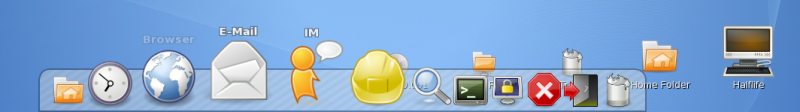
\includegraphics[width=0.5\hsize]{image200611/cairo-dock-ss.png}
	\end{center}

	Debian では\footnote{パッケージを管理している他のディストリビューションでも使われています。}
	開発元、オリジナル配布元のことを Upstream といいます。

\begin{enumerate}

	\item パッケージ化を行うためにパッケージをインストールします。
	\\
	\begin{commandline}
# apt-get install dh-make devscripts debhelper dpkg-dev dpatch 
	\end{commandline}
	\\
	\item ソフトウェアのソースコードをダウンロードし、展開します。
		
	\begin{commandline}
% wget http://www.gnome-dock.org/prerelease/cairo-dock-0.0.1b.tar.gz
% tar -xzf cairo-dock-0.0.01b.tar.gz
	\end{commandline}
		\\
	\item 展開した後、ディレクトリ名を パッケージ名-パッケージのバージョン になるように修正します。

	\begin{commandline}
% ls -l 
drwxr-xr-x  2 iwamatsu iwamatsu    1024 2006-08-09 01:29 cairo-dock
-rw-r--r--  1 iwamatsu iwamatsu  107560 2006-08-09 01:30 cairo-dock-0.0.1b.tar.gz

% mv cairo-dock cairo-dock-0.0.1b
	\end{commandline}

		すでに行われている場合は行う必要はありません。

	\item バックアップファイルや実行ファイルが残っているので、消しておきます。

	\begin{commandline}
% ls
Makefile       clock.svg        folder.svg         lowfat.svg           start-cairo-dock.sh~  terminal.svg
cairo-dock     configure.scan   gnome-fs-home.svg  movies.svg           sticky-notes.svg      user-home.svg
cairo-dock.c   development.svg  im.svg             music.svg            stop.svg              user-trash-full.svg
cairo-dock.c~  editor.svg       lockscreen.svg     search.svg           tango-colors.h        web-browser.svg
chat.svg       email.svg        logout.svg         start-cairo-dock.sh  tango-colors.h~
% make clean
	\end{commandline}
	\item 対象のソフトウェアのディレクトリに移動し、dh\_make --createorigを実行します。

		dh\_make を実行したときに、パッケージの種類を選択します。
		\begin{itemize}
			\item single binary

				ひとつのバイナリパッケージを作成する。
			\item multiple binary
				
				複数のバイナリパッケージを作成する。
			\item library

				ライブラリ用のパッケージを作成する。
			\item kernel module
		
				カーネルモジュール用のパッケージを作成する。
			\item cdbs
		
				cdbs ( Common Debian Build System ) を使ったパッケージを作成する。
		\end{itemize}
		

		実行すると、debian ディレクトリが作成されます。
		\texttt{--createorig} を指定しない場合はオリジナル用のディレクトリ( 今回の場合は cairo-dock-0.0.1b.orig )が作成されません。
		このディレクトリがない場合は、ソースパッケージの一部として配布される .orig.tar.gz が生成されません。

	\begin{commandline}
% dh_make --createorig

Type of package: single binary, multiple binary, library, kernel module or cdbs?
 [s/m/l/k/b] s

Maintainer name : Nobuhiro Iwamatsu
Email-Address   : hemamu@t-base.ne.jp
Date            : Fri, 17 Nov 2006 07:30:18 +0900
Package Name    : cairo-dock
Version         : 0.0.1b
License         : blank
Type of Package : Single
Hit <enter> to confirm:
Done. Please edit the files in the debian/ subdirectory now. You should also
check that the cairo-dock Makefiles install into $DESTDIR and not in / .
	\end{commandline}
	
	\item debianディレクトリ内を編集します。

		dh\_make を行ったあとの debian ディレクトリは以下のようになっています。
		これらはテンプレートファイルなので、パッケージによって必要のないものも含まれています。
		\begin{itemize}
			\item README.Debian

				Debian 固有のREADME			           
			\item changelog
  
				Debian 固有の変更履歴
			\item copyright
 
				ソフトウェアのライセンスとコピーライト 
			\item docs    
            
				\texttt{/usr/share/doc} にインストールされるファイルのリスト
			\item emacsen-startup.ex
			\item emacsen-install.ex
			\item emacsen-remove.ex
       
 				xemacs 用テンプレート
			\item postinst.ex
			\item postrm.ex
			\item preinst.ex         
			\item prerm.ex

				インストール、アンインストール時に実行されるスクリプトテンプレート
			\item cairo-dock-default.ex
  
				\texttt{/etc/init.d/}用のテンプレート

			\item compat     
			\item cron.d.ex
  
				crond 用のテンプレート
			\item init.d.ex
           
				\texttt{/etc/init.d/}用のテンプレート
			\item rules

				パッケージ作成用 Makefile
			\item cairo-dock.doc-base.EX  

				docbook 用のテンプレート
			\item control
    
				パッケージのメタ情報
			\item dirs
			\item manpage.xml.ex 
			\item manpage.sgml.ex       
			\item manpage.1.ex
        
				manpages のテンプレート
			\item menu.ex
          
				menu システム用テンプレート
			\item watch.ex

				upstream 監視用設定テンプレート
		\end{itemize}
		
		
	\item *.ex および *.EX ファイルを削除します。

		今回のソフトウェアのパッケージ化には *.ex や *.EX は必要ないので、削除します。
 
	\item control ファイルの編集

		control ファイルを編集します。
	\begin{itemize}
		\item Source	

			ソースパッケージ名を記述します。
			今回は ソースの名前から cairo-dock とします。

			詳細は Debian-Policy の {\bf 5.6.1 Source} を参照してください。
		\item Section

			パッケージの種類を指定します。
			cairo-dock は x11 用のソフトウェアなので、x11 とします。

			詳細は Debian-Policy の {\bf 2.4 Sections} を参照してください。
		\item Priority
	
			パッケージの優先度を指定します。
			今回のパッケージは特に重要でもないので、optional を指定します。

			詳細は Debian-Policy の {\bf 2.5 Priorities} を参照してください。

		\item Maintainer

			パッケージメンテナ名とメールアドレスを指定します。
			私がメンテナンスしますので、私の名前(ローマ字)と連絡用のメールアドレスを
			記述します。

			詳細は Debian-Policy の {\bf 5.6.2 Maintainer} を参照してください。
			
		\item Build-Depends
			
			パッケージをコンパイルするために依存するパッケージを指定します。
			依存しているパッケージを調べるためには \texttt{configure -h} で指定可能なオプションから調べたり、
			ヘッダファイルやコンパイルエラーメッセージなどから調べるといいでしょう。

			詳細は Debian-Policy の {\bf 7.6 Relationships between source and binary packages} を参照してください。
		\item Standards-Version

			Debian Policy バージョンを指定します。

			詳細は Debian-Policy の {\bf 5.6.11 Standards-Version} を参照してください。
		\item Package

			バイナリパッケージ名を指定します。今回は cairo-dock となります。

			詳細は Debian-Policy の {\bf 5.6.7 Package} を参照してください。
		\item Architecture

			アーキテクチャ依存(any/各アーキテクチャ)、非依存(all)の指定を行います。

			詳細は Debian-Policy の {\bf 5.6.8 Architecture} を参照してください。

		\item Depends,Recommends,Suggests,Conflicts,Provides,Replaces

			パッケージの依存関係を記述します。
			
			詳細は Debian-Policy の {\bf .6.10 Package interrelationship fields} を参照してください。
		\item Description
			パッケージの簡単な説明と詳細な説明を記述します。

			詳細は Debian-Policy の {\bf 5.6.13 Description} を参照してください。
	\end{itemize}

		以下が今回のパッケージの control ファイルです。

		\begin{commandline}
Source: cairo-dock
Section: x11
Priority: optional
Maintainer: Nobuhiro Iwamatsu <hemamu@t-base.ne.jp>
Build-Depends: debhelper (>= 5) ,libcairo2-dev ,libgtk2.0-dev ,librsvg2-dev ,libglitz-glx1-dev
Standards-Version: 3.7.2
		
Package: cairo-dock
Architecture: any
Depends: ${shlibs:Depends}, ${misc:Depends}
Description: Dock application like dock of MacOS X
 cairo-dock is dock application like dock of MacOS X.
 This reproduces dock of MacOS X by using Xgl/Compiz and Xcompmgr.

		\end{commandline}
		\\
	\item copyright の変更

		Upstreamのコピーライト、ソフトウェアのライセンス、パッケージのコピーライト、Upstreamのソース取得先
		を記述します。\\
		Upsteam のコピーライトはソースに含まれている(場合がある) COPYING 
		ファイルやWeb サイトを参照にするといいでしょう。
		ソフトウェアのライセンスに関しては、ソースに含まれている(場合がある)COPYING ファイルや LICENCE ファイル
		を参照するといいでしょう。たまにソフトウェアのライセンスが書いていない場合があります。このときは開発者に
		連絡を取り、ライセンスを確認する必要があります。

		Debian-Policy の {\bf 12.5 Copyright information} を参照してください。
		
		\begin{commandline}
Package Maintainers:
Nobuhiro Iwamatsu <hemamu@t-base.ne.jp> from Thu,  9 Nov 2006 00:19:36 +0900.

Upstream Authors:

Mirco "MacSlow" Mueller <macslow@bangang.de>
Behdad Esfahbod <behdad@behdad.org>
David Reveman <davidr@novell.com>
Karl Lattimer <karl@qdh.org.uk>

Upstream Website:  <http://www.gnome-dock.org/trac>

Copyright:

Mirco "MacSlow" Mueller <macslow@bangang.de>
Behdad Esfahbod <behdad@behdad.org>
David Reveman <davidr@novell.com>
Karl Lattimer <karl@qdh.org.uk>

This program is free software; you can redistribute it and/or
modify it under the terms of the GNU General Public License
as published by the Free Software Foundation; either version 2
of the License, or (at your option) any later version.

This program is distributed in the hope that it will be useful,
but WITHOUT ANY WARRANTY; without even the implied warranty of
MERCHANTABILITY or FITNESS FOR A PARTICULAR PURPOSE.  See the
GNU General Public License for more details.

You should have received a copy of the GNU General Public License
along with this program; if not, you can either send email to this
program's maintainer or write to: The Free Software Foundation,
Inc.; 51 Franklin Street, Fifth Floor, Boston, MA 02110-1301, USA.

On Debian systems, a copy of the license can be found in /usr/share/common-licenses/GPL
		\end{commandline}
		\\
	\item changelog の修正
		Debian 特有の変更点を changelog に記録する必要があります。
		エディタ等で修正することも可能ですが、dch というフロントエンドが用意されていますので、
		これを使って changelog を編集します。

	\begin{center}
		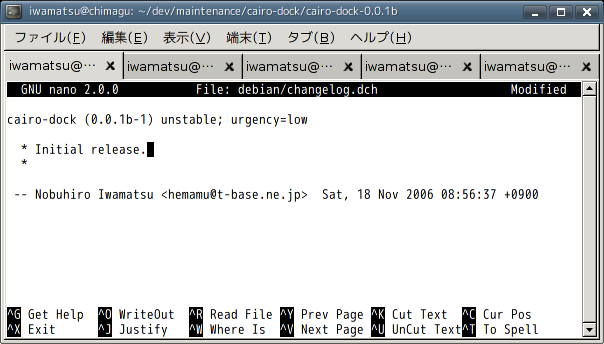
\includegraphics[width=0.5\hsize]{image200611/dch_image.png}
	\end{center}

	\item Upstream のソース変更

		そのままのソースコードでは パッケージ化した場合に不都合がある場合が多々あります。
		パッケージを作成する前に、Debian のパッケージ作成に合うように修正する必要があります。

		今回修正した点は以下のとおりです。

		\begin{itemize}
			\item Makefile の install ターゲットがないので追加します。
			\item Debian で配布されている libcarioパッケージの cairo-glitzが有効になってないので、
				Makefile の \texttt{-DHAVE\_GLITZ} を無効にします。

		変更前\\
		\begin{commandline}
APP = cairo-dock

CFLAGS  = `pkg-config --cflags cairo gtk+-2.0 librsvg-2.0 glitz-glx` -DHAVE_GLITZ
LDFLAGS = `pkg-config --libs   cairo gtk+-2.0 librsvg-2.0 glitz-glx` -lm

SRC = cairo-dock.c

all: $(APP)

clean:
        rm -f *.o *~ $(APP)
		\end{commandline}
		\\
		変更後\\
		\begin{commandline}
APP?=cairo-dock
BINDIR?=/usr/bin

CFLAGS  = `pkg-config --cflags cairo gtk+-2.0 librsvg-2.0 glitz-glx`
LDFLAGS = `pkg-config --libs   cairo gtk+-2.0 librsvg-2.0 glitz-glx` -lm

SRC = cairo-dock.c

all: $(APP)

clean:
        rm -f *.o *~ $(APP)

install:
        install -d ${DESTDIR}${BINDIR}
        install -m 755 cairo-dock ${DESTDIR}${BINDIR}

		\end{commandline}

			\item cairo-dock.c の画像ファイルの指定がプログラムのあるディレクトリになっているので修正します。


		\end{itemize} 


		直接ソース等を修正してもいいのですが、差分で管理するために diff を取り、dpatch で管理します。
		詳細は Debian 勉強会 2005年07月の資料\footnote{debianmeetingresume200507.pdf}にあります。

	\subsubsection{manpage の作成}		

		実行権限があるファイルに manpage がない場合作成し、パッケージで提供する必要があります。
				
	\item パッケージの作成

		debuild コマンドを使い、パッケージを作成します。

		\begin{commandline}
% debuild
 fakeroot debian/rules clean
dh_testdir
dh_testroot
rm -f build-stamp configure-stamp
# Add here commands to clean up after the build process.
/usr/bin/make clean
make[1]: ディレクトリ `/tmp/cairo-dock-0.0.1b' に入ります
rm -f *.o *~ cairo-dock
make[1]: ディレクトリ `/tmp/cairo-dock-0.0.1b' から出ます
dh_clean
 dpkg-source -b cairo-dock-0.0.1b
dpkg-source: building cairo-dock using existing cairo-dock_0.0.1b.orig.tar.gz
dpkg-source: building cairo-dock in cairo-dock_0.0.1b-1.diff.gz
dpkg-source: building cairo-dock in cairo-dock_0.0.1b-1.dsc
 debian/rules build
dh_testdir
# Add here commands to configure the package.
touch configure-stamp
dh_testdir
# Add here commands to compile the package.
/usr/bin/make
make[1]: ディレクトリ `/tmp/cairo-dock-0.0.1b' に入ります
cc `pkg-config --cflags cairo gtk+-2.0 librsvg-2.0 glitz-glx`   
	`pkg-config --libs   cairo gtk+-2.0 librsvg-2.0 glitz-glx` -lm  cairo-dock.c   -o cairo-dock
make[1]: ディレクトリ `/tmp/cairo-dock-0.0.1b' から出ます
#docbook-to-man debian/cairo-dock.sgml > cairo-dock.1
touch build-stamp
 fakeroot debian/rules binary
dh_testdir
dh_testroot
dh_clean -k
dh_installdirs
# Add here commands to install the package into debian/cairo-dock.
/usr/bin/make DESTDIR=/tmp/cairo-dock-0.0.1b/debian/cairo-dock install
make[1]: ディレクトリ `/tmp/cairo-dock-0.0.1b' に入ります
install -d /tmp/cairo-dock-0.0.1b/debian/cairo-dock/usr/bin
install -m 755 cairo-dock /tmp/cairo-dock-0.0.1b/debian/cairo-dock/usr/bin
install -d /tmp/cairo-dock-0.0.1b/debian/cairo-dock/usr/share/cairo-dock
install -m 666 *.svg /tmp/cairo-dock-0.0.1b/debian/cairo-dock/usr/share/cairo-dock
make[1]: ディレクトリ `/tmp/cairo-dock-0.0.1b' から出ます
dh_testdir
dh_testroot
dh_installchangelogs
dh_installdocs
dh_installexamples
dh_installman
dh_link
dh_strip
dh_compress
dh_fixperms
dh_installdeb
dh_shlibdeps
dh_gencontrol
dpkg-gencontrol: warning: unknown substitution variable ${misc:Depends}
dh_md5sums
dh_builddeb
dpkg-deb: `../cairo-dock_0.0.1b-1_i386.deb' にパッケージ `cairo-dock' を構築しています。
 dpkg-genchanges
dpkg-genchanges: including full source code in upload
dpkg-buildpackage (debuild emulation): full upload (original source is included)
Now running lintian...
W: cairo-dock: description-synopsis-might-not-be-phrased-properly
W: cairo-dock: wrong-bug-number-in-closes l3:#nnnn
Finished running lintian.
Now signing changes and any dsc files...
 signfile cairo-dock_0.0.1b-1.dsc Nobuhiro Iwamatsu <hemamu@t-base.ne.jp>

次のユーザーの秘密鍵のロックを解除するには
パスフレーズがいります:“Nobuhiro Iwamatsu <hemamu@t-base.ne.jp>”
1024ビットDSA鍵, ID 3170EBE9作成日付は2003-09-29


 signfile cairo-dock_0.0.1b-1_i386.changes Nobuhiro Iwamatsu <hemamu@t-base.ne.jp>

次のユーザーの秘密鍵のロックを解除するには
パスフレーズがいります:“Nobuhiro Iwamatsu <hemamu@t-base.ne.jp>”
1024ビットDSA鍵, ID 3170EBE9作成日付は2003-09-29


Successfully signed dsc and changes files

		\end{commandline}

	\end{enumerate}

\subsection{パッケージのテスト}
	パッケージができたから終わりなのではなく、できたパッケージの動作確認やパッケージ段階で不具合がないか、確認する必要があります。
	
	\subsubsection{pbuilder でビルドチェック}

		pbuilder\footnote{http://packages.qa.debian.org/p/pbuilder.html} は chrootシステムを構築し、その中でパッケージのビルドを行うツールです。
		最低限のユーザーランドの上で、パッケージの依存関係を解決し、パッケージをビルドできるの確認することができます。
		パッケージの依存関係に不備があった場合はパッケージがビルドできません。パッケージはできたが、実は自分の環境でしか
		ビルドできなかったという単純な問題を無くすために使用したほうがいいでしょう。

	\subsubsection{実際にインストールして、動作確認を行う}

		動作確認していないものを不特定多数の人に配布するのは問題ですので(やってない人もおられるようですが。)実際にインストール
		して、動作確認を行います。

		\begin{commandline}
# dpkg -i cairo-dock_0.0.1b-1_i386.deb
% cairo-dock 
		\end{commandline}

	\subsubsection{アンインストールできるか確認する}

		インストールした際にアンインストールスクリプトに不具合があり、正常にアンインストールできない
		場合があります。アンインストールもできるか確認します。

\subsection{まとめ}
	Debian パッケージを作成することは難しくなく、容易に作成できる環境は整っています。
	
	肝心なのはツールを使えるようになることではなく、Debian Policy をどれだけ熟読しているか、
	にかかってくるように思います。
	
	作って分からないことがあれば debian-devel@jp\footnote{\texttt{debian-devel@debian.or.jp}}等で聞くといいでしょう。	
	

\dancersection{sid を日常環境として使うための注意}{上川}
\label{sec:YYY}

\subsection{sid とはなにものか}

Debian sid は別名 unstable で、毎日リリースされている Debian の開発版で
す。開発者が新しいパッケージをリリースしたらまずそこに入ります。毎日日本
時間午前4時くらいに処理されており、そのタイミングで新しいバージョンが配
布されます。

開発者に近い層のユーザは、最新版のパッケージを利用するために unstable を
利用します。問題があれば随時バグ報告をしていきます。また、apt-listbugs
などを利用し、他のユーザから報告された深刻なバグがないか確認しながら作業
します。


\subsection{インストール方法}

毎日最新版になるので、安定して直接インストールできる方法というのは基本的
には無いでしょう。安定版をインストールしてから、 sid にアップグレードす
るという形が通常のやりかたです。

また、別の方法として、chroot 内部に sid を飼うという方法があります。
debootstrap や、 cdebootstrap などのツールを利用すると、 chroot 内部で
Debian sid が稼働している状況をつくれます。pbuilder などのツールを利用す
るとより便利に利用できます。

sid は最新版を常においかけているので、深刻なバグのリスクに出会う危険性が
常にあります。 chroot 内部で常に最新版を確認して、それを外部に展開すると
いうやりかたをしないと危険でしょう。

\subsection{魅力}

常に最新版が利用できます。開発が起きている場です。開発をしたいだとか、オー
プンソースの世界の動きを肌で感じたいというのであれば、お薦めです。

\subsection{情報源}

IRC や ML や勉強会で情報収集しましょう。
\verb!#debian-devel! IRCチャンネルのトピックが一番最新の情報が得られます。

apt-listbugs や apt-listchanges というツールも利用しましょう。
apt-listbugs は今インストールしようとしているパッケージのバージョンに該
当する深刻なバグレポートを表示してくれるツールです。apt-listchanges は
前回インストールしたバージョンからの changelog の差分を表示してくれるツー
ルです。

\dancersection{bugreport 論}{上川}

\subsection{Debian BTS の特徴}

Debian BTS は、ウェブとメールフロントエンドをもつバグトラッキングシステ
ムです。他のバグトラッキングシステムと違う点として、操作が全てメールでし
かできないという点と、情報が全て完全に公開されるという点があります。
また、バグレポートをパッケージ単位で分類しているという点も特徴です。

\subsection{使われ方}

深刻なバグ(RC バグ)を登録すると、そのパッケージのバージョンはリリース
できない、という意味になります。各ユーザはapt-listbugs を経由してそのよ
うなバグを確認し、深刻なバグのあるパッケージのバージョンをインストールし
ないように回避できます。また、この情報はリリースマネージメントにつかわれ
ています。

\subsection{アーキテクチャ}

バックエンドデータベースはプレーンのテキストファイルです。ファイル構造は
下記のようになっています。

\begin{itemize}
 \item /org/bugs.debian.org/spool
       \begin{itemize}
	\item incoming/
	\item db-h/
	      \begin{itemize}
	       \item 00/
		     \begin{itemize}
		      \item ..
		      \item 314200.log
		      \item 314200.report
		      \item 314200.status
		      \item 314200.summary
		     \end{itemize}
	       \item ..
	       \item 99/
	      \end{itemize}
	\item archive/
	      \begin{itemize}
	       \item 00/
	       \item ..
	       \item 99/
	      \end{itemize}
	\item index.db -- index.db.realtimeへのシンボリックリンク
	\item index.archive -- index.archive.realtimeへのシンボリックリ
	      ンク
	\item nextnumber
       \end{itemize}
\end{itemize}

メールを受信したら、そのメールが incoming 以下にスプールされます。
そのメールを15分に一回 cron から起動されるスクリプトが処理します。


ウェブ経由でバグ報告を確認するためのcgi があります。その cgi 経由では 
BTS は内容の閲覧だけができ、変更はしません。

また、スクリプトなどから利用するために、SOAP のフロントエンドがあります。
ドキュメントは一行もありません。

現状 \url{http://bugs.donarmstrong.com/cgi-bin/soap.cgi} でステージング
されています。今後は \url{http://bugs.debian.org} に移行したいようです。
ネームスペースは\texttt{Debbugs/SOAP/Status}で、そこで\verb!get_status!とい
う関数が定義されています。\verb!get_status!は複数の数字パラメータをうけ、
そのあたえられた数字に対応するバグレポートの情報をかえします。
\verb!get_status!は、バグ報告の本文ではなく、メタデータを返します。


\subsection{文化}

たまに BSP などの祭があります。バグトラッキングシステムに登録されている
バグで最初に対応されないものについては、そのまま放置され時間だけが過ぎて
しまう傾向があります。それらに対して新たな気持ちで対応しようというもので
す。

\subsection{参考文献}

\begin{itemize}
 \item Debian勉強会 2005年10月資料 「debbugs internal」
 \item Debian勉強会 2005年10月資料 「apt-listbugs の生い立ちと実装」
 \item \texttt{/usr/share/doc/debian/bug-maint-mailcontrol.txt}など
\end{itemize}


\newpage
\dancersection{Debian Weekly News trivia quiz}{上川 純一}

ところで、Debian Weekly News (DWN)は読んでいますか?
Debian 界隈でおきていることについて書いているDebian Weekly News.
毎回読んでいるといろいろと分かって来ますが、一人で読んでいても、解説が少
ないので、
意味がわからないところもあるかも知れません。みんなでDWNを読んでみましょう。

漫然と読むだけではおもしろくないので、DWNの記事から出題した以下の質問にこたえてみてください。
後で内容は解説します。



\subsection{2006年25号}
\url{http://www.debian.org/News/weekly/2006/25/}
にある6月20日版です。

\santaku
{Isaac Clerencia さんは、スペイン
のサラゴサ市当局が、6 ヶ所ある場所に Debian ベースのシンク
ライアントを設置したと報告しました。その場所とはどこでしょうか}
{ラーメン屋}
{コンビニエンスストア}
{老人ホーム}
{C}

\santaku
{Yaroslav Halchenkoさんが Debian Packge 内のあるファイルが圧縮されていて、読むことが出来ないと気がつきました。
そのファイルとは何でしょうか。}
{Word ファイル}
{PDF ファイル}
{SREC ファイル}
{B}

\subsection{2006年26号}
\url{http://www.debian.org/News/weekly/2006/26/}
にある6月27日版です。

\santaku
{9月にイタリアのある都市でDebian コミュニティカンファレンスがおこなわれます。
そのある都市とはどこでしょう。}
{ベニス}
{デセンツァーノ・デル・ガルーダ}
{カリブ島}
{A}

\santaku
{最近セキュリティチームのメンバーが増えました。それはだれでしょうか。}
{Steve Kemp}
{Hidehazu Koiwa}
{Andreas Barth}
{A}

\subsection{2006年27号}
\url{http://www.debian.org/News/weekly/2006/27/}
にある7月4日版です。
\santaku
{最近また新しいOSにDebianを移植している噂があるらしい。それはどのOSか?}
{Plan9}
{Minix3}
{Mona}
{B}

\santaku
{Paul Wise さんがあたらしいグループを作成しました。それはどのグループか?}
{debian-smoker}
{debian-soccer}
{debian-flash}
{C}


\subsection{2006年28号}
\url{http://www.debian.org/News/weekly/2006/28/}
にある7月11日版です。

\santaku
{Matthew Garret はなにを断言したか}
{Debian に貢献していない者には Debian に要求する権利は無い}
{あれげはあれげ}
{人生いろいろ}
{A}

\subsection{2006年29号}
\url{http://www.debian.org/News/weekly/2006/29/}
にある7月18日版です。

\santaku
{7月に不正侵入されたサーバはどれか?}
{gluck.debian.org}
{ftp-master.debian.org}
{hanzubon.jp}
{A}

\santaku
{上川が発表したのは何か?}
{あれげハック}
{pbuilder やめます宣言}
{Intel Mac 向けの Debian サポートの進捗}
{C}


\subsection{2006年30号}
\url{http://www.debian.org/News/weekly/2006/30/}
にある7月25日版です。

\santaku
{ブータンの公用語向けのDebianは}
{HondaLinux}
{BongaLinux}
{DzongkhaLinux}
{C}
\subsection{2006年31号}
\url{http://www.debian.org/News/weekly/2006/31/}
にある8月1日版です。

\santaku
{Debianパッケージ内のドキュメントはビルド時にビルドするべきか?}
{ビルドするのに時間かかるからコンパイル済のものをいれるべき}
{アーキテクチャ非依存としてビルドするべき}
{アーキテクチャ依存としてビルドするべき}
{B}

\subsection{2006年32号}
\url{http://www.debian.org/News/weekly/2006/32/}
にある8月8日版です。

\santaku
{SPIの理事長は?}
{Neil McGovern }
{Bdale Garbee}
{Michael Schultheiss}
{B}

\subsection{2006年33号}
\url{http://www.debian.org/News/weekly/2006/33/}
にある8月15日版です。

\santaku
{Martin Krafft がアーカイブソフトウェアについて発表したのは?}
{チルダがサポートされた}
{古いバージョンは自動で削除するようになった}
{セキュリティーアップデートの速度がはやくなった}
{A}

\subsection{2006年34号}
\url{http://www.debian.org/News/weekly/2006/34/}
にある8月22日版です。

\santaku
{Debian をサポートするというプレスリリースを出した会社は?}
{HP}
{IBM}
{Ubuntu}
{A}

\subsection{2006年35号}
\url{http://www.debian.org/News/weekly/2006/35/}
にある8月29日版です。

\santaku
{Alexander WirtがFrOSConのために準備したのは?}
{ぐるぐるの形をした金メダル}
{ぐるぐるの形をしたプレッツェル}
{ぐるぐるの形をしたぐるぐる}
{B}

\subsection{2006年36号}
\url{http://www.debian.org/News/weekly/2006/36/}
にある9月5日版です。

\santaku
{Joerg Jaspertが発表した新しいツールは}
{cdrkit}
{cdrecord}
{dvdrecord}
{A}
\subsection{2006年37号}
\url{http://www.debian.org/News/weekly/2006/37/}
にある9月12日版です。

\santaku
{Anthony Towns が提案したのは}
{BTSでのライセンス関連の問題についてタグをつけること}
{あらゆるライセンス問題はなかったことにすること}
{ライセンスなんて所詮ただの文章さ}
{A}


\subsection{2006年38号}
\url{http://www.debian.org/News/weekly/2006/38/}
にある9月19日版です。

\santaku
{Josselin Mouette が GNOME 2.16 について説明したのは}
{stable へのバックポート}
{experimental への投入}
{unstable への投入}
{B}

\santaku
{Russel Coker が議論する際の道具として提案したのは?}
{意味の無い議論をベイジアンフィルタではじく}
{killfile の積極的な活用}
{議論のサマリをまとめるためのwikiの利用}
{C}

\santaku
{最近 Debian にはいったパッケージである「ttf-vlgothic」のvlはどういう意味か?}
{ディストリビューションの名前}
{私の名前はやまねです。}
{very local }
{A}


\subsection{2006年39号}
\url{http://www.debian.org/News/weekly/2006/39/}
にある9月26日版です。

\santaku
{プロジェクトリーダーを罷免する決議が出たのはなぜか?}
{Dunk-Tank プロジェクトを発足したから}
{やるきがまったくみられないから}
{タイの政変の影響}
{A}

\santaku
{一般決議に関しての規則がかわったのはなぜか}
{現在多数提起されているから}
{くだらないものが提起されすぎだから}
{Dunk-Tank が気に入らないから}
{A}

\subsection{2006年40号}
\url{http://www.debian.org/News/weekly/2006/40/}
にある10月31日版です。

\santaku
{Frank K\"usterがカーネル 2.6.18 パッケージについて発表したのは?}
{まだ安定していないけどどんどん利用してください}
{General Resolution の結果、 Linuxじゃないカーネルを今後利用する}
{firmware blob を Debian package に含めるようにした}
{C}

\santaku
{mplayer パッケージになにがおきたか?}
{NEW キュー滞在時間の新記録をさらに更新した}
{Debian unstable に入った}
{もうあきらめることになった}
{B}


%以上 11月まで

\newpage{}

\dancersection{Debian Weekly News 問題回答}{上川}
%\twocolumn

Debian Weekly News の問題回答です。
あなたは何問わかりましたか?
%回答はdebianmeetingresume2006-fuyu.jqzというファイルに生成されるので、
%それを手動でコピペして使う。
\\
% ここからコピペ
1. C\\
2. B\\
3. A\\
4. A\\
5. B\\
6. C\\
7. A\\
8. A\\
9. C\\
10. C\\
11. B\\
12. B\\
13. A\\
14. A\\
15. B\\
16. A\\
17. A\\
18. B\\
19. C\\
20. A\\
21. A\\
22. A\\
23. C\\
24. B\\
\onecolumn
\newpage

\vspace*{15cm}
\hrule
\vspace{2mm}

\includegraphics[width=2cm]{image200502/openlogo-nd.eps}
\noindent \Large \bf あんどきゅめんてっど でびあん 2006年冬号\\ \\
\noindent \normalfont 2006年12月30日 \hspace{5mm}  初版第1刷発行\\
\noindent \normalfont 東京エリア Debian 勉強会 (編集・印刷・発行)\\
\hrule

\end{document}
